
% ===============================================================
% =						System Description						=
% ===============================================================
\chapter{System Description and Functionalities}
\label{cha:system}

This chapter describes the most relevant aspects related to the development of the system such as the concept behind the application, the architecture and general structure. It includes a detailed explanation about the functionalities implemented with the proposed technologies and the preliminary user interfaces.

\section{System Description}
\label{sec:system_description}

\todo[inline]{Para rever}
Photo aesthetic quality assessment aims to classify the photographs into high or low quality automatically. \citeauthor{tong2005classification} \cite{tong2005classification} attempted to classify photographs into those taken by professionals or casual users using low-level features derived from computer vision techniques. As already mentioned in Section \ref{subsub:eval_features}, techniques for training classifiers to automatically assess the quality of an image, have already been devised. Since mobile devices are constantly used in photography nowadays, it is only logical that improving photography in such devices is the next step to take.

\subsection{Concept}
The development of this set of features started by thinking of useful information that could be extracted from a real-time camera feed. The purpose of extracting this information, is to give a user a different insight of the photo that is being taken and help to attain better results without resorting to any photo manipulation techniques or tools. It results in an application that demonstrates a set of tools and techniques that process real-time images and responds with visual cues overlaid on the processed data.

These visual cues have as an objective to identify key elements in an image, such as colour information. Colours have already been identified as an important factor in a photograph (Section \ref{subsub:colour_balance}). Therefore, understanding the colour composition and pureness of the colours is useful for a user to study the composition and rearrange the colours before even taking the photo. The same applies when talking about the composition of the elements. As an example, identifying the main object or detect faces may be useful for testing various compositions in an attempt to find the best one.

With this idea in mind, we gathered a number of features that we though to give useful information when taking a photograph. Some of these features are related to the colours being displayed. We devised a couple of histograms to visualize the distribution amount of each colour, as well as a saturation detector for detecting when the scenario has a colours with a low level of pureness. Other features more related to the composition of the photo were implemented, such as face detection and object detection through segmentation, detection of the horizon line when photographing a seascape or landscape, detection of main lines which have an important role when guiding the viewer in a photo, detection of the line of symmetry and testing the balance between the elements in an image. With the main purpose of obtaining the best aesthetic results without any image editing, we also implemented a couple of metrics regarding the simplicity of an image and number of colours used. Later in these sections, these features will be described in detail and discussed regarding the way the result is displayed and the general behaviour of the algorithms.

\subsection{Architecture}

Figure \ref{fig:sys_diagram} illustrates the architecture chosen for this project which is based on mechanisms offered by the Android operating system. The system starts by receiving data from the device's camera, and pass it to the \emph{CameraViewer}. This object, besides controlling which feature is enabled, also controls the camera and serves as a gate since it receives all input data and reliably redistributes to the objects controlling each enabled feature. 
At this stage, it passes through various \emph{wrapper} objects. Each object is responsible for wrapping the data and send them to the Java Native Interface (\emph{JNI}) where all algorithms are run with the help of \emph{OpenCV}. All the results are then sent back to the object responsible for each feature. The last stage is the Presentation stage where all results of the algorithms are post-processed and the visual information is updated and shown to the user through the viewfinder.

\begin{figure}[htb]
	\centering
	\includegraphics[width=\textwidth]{interface/sys_diagrama.pdf}
	\caption{Architecture of the system.}
	\label{fig:sys_diagram}
\end{figure}

Each feature has its wrapper as well as presentation stage. The Presentation stage was implemented only in Android and all the visual cues work as an overlay over the current camera's live-feed, so that the user can have an immediate response to what she is seeing. Figure \ref{fig:class_diagram} illustrates a class diagram with the dependencies of each feature, were all that is drawn is an overlay and has its own implementation. Each feature must extend the \emph{Overlay} class, therefore it can be drawn in the viewfinder since the \emph{Overlay} itself extends the default Android class \emph{View}.

\begin{figure}[htb]
	\centering
	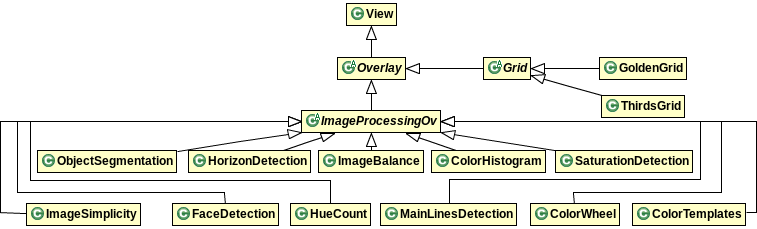
\includegraphics[width=\textwidth]{interface/diagrama.png}
	\caption{Class diagram of the Presentation stage in Figure \ref{fig:sys_diagram}.}
	\label{fig:class_diagram}
\end{figure}

Still in the presentation stage, to alternate between features we devised a simple interface dividing coupling the similar ones. Figure \ref{fig:app_menu} shows the interface, which consists of a list of the implemented features. To use a feature, the user simply has to tap on a checkbox to start the algorithm which also allows to use multiple features at the same time. Such a simple interface was chosen to keep the viewfinder cleaner and due to the lack of icons that accurately represent what each feature is supposed to do.
\begin{figure}[htb]
	\centering
	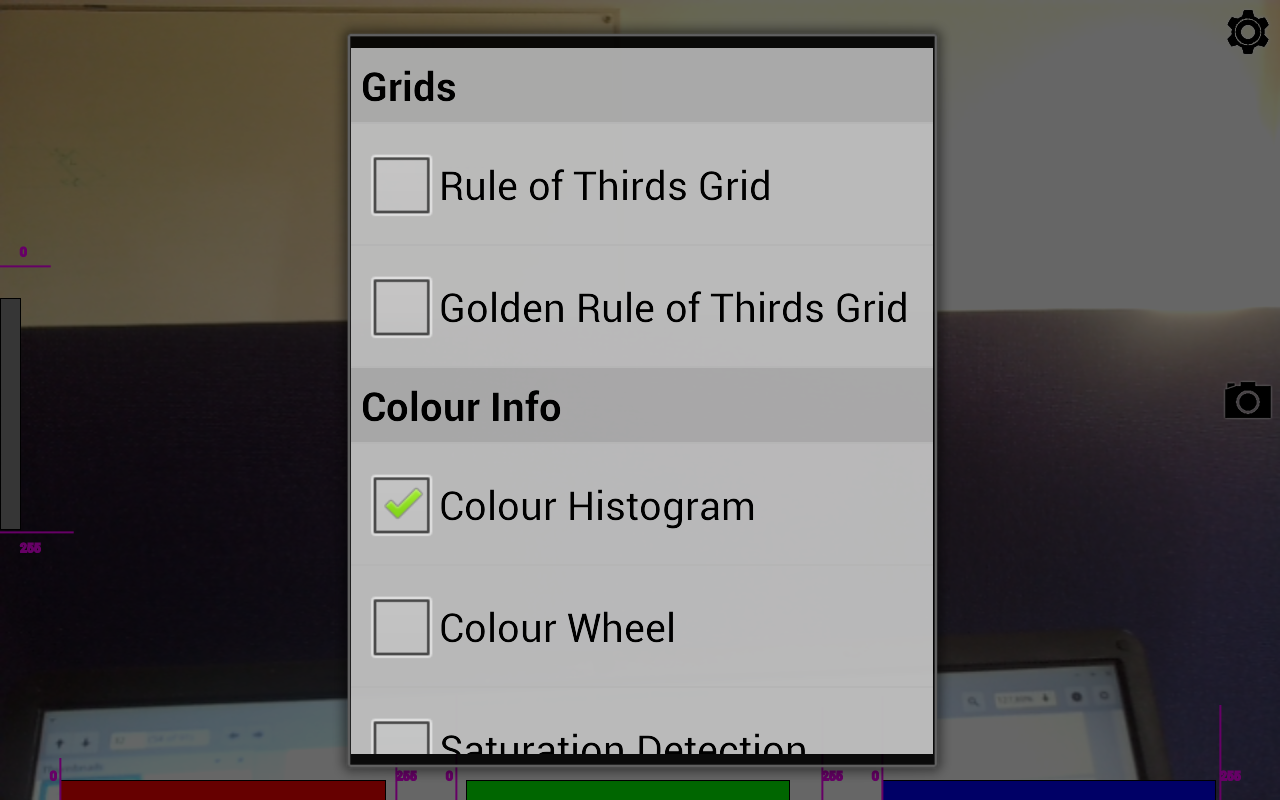
\includegraphics[width=0.5\textwidth]{interface/menu.png}
	\caption{Menu to select each feature.}
	\label{fig:app_menu}
\end{figure}


The JNI stage is composed by all the algorithms implemented. This stage is where the Android's Java Virtual Machine calls native applications which can be programmed for the hardware, or libraries that were written in other languages such as \emph{C} or \emph{C++}. In the context of this thesis, we created our own native library in \emph{C++} complemented by the library \emph{OpenCV} which, by itself, already includes several hundreds of computer vision algorithms. Although we used static classes instead of objects, our native library as a class for each feature, in resemblance to the class diagram in Figure \ref{fig:class_diagram}.

\section{Functionalities}
\label{sec:functionalities}

This section describes in detail the functionalities and experiments implemented in the proposed system. The set of functionalities implemented were considered to be more interesting to explore in a real-time environment than the usual set of features already presented in regular camera applications or digital cameras.

\subsection{Colour Histograms and Average Saturation}
\label{sub:histograms}

Colour histograms have been used for a long time in image processing and photography to measure the distribution of colours. A colour histogram represents the number of pixels in each of a fixed list of colour ranges, that span the image's colour space, the set of all possible colours.

These can be built in any kind of colour space and have multiple dimensions depending on the number of measurements taken, although it is normally used to count the number of pixels for three-dimensional colour spaces.

The visualization of such information becomes really important when colour is one of the elements in which photography is most focused on. \citeauthor{bertin1983semiology} stated that in the field of information visualization, colour has historically been used as one of the primary visual variables through which difference in data can be distinguished and is considered as one of the fundamental building blocks of visualizations today.

Exploring the importance of colour, in \cite{haber2011colourvis} colour information is visualized with a variation of a stacked line graph visualization, which give the viewer a sense of the colours and the amount of each colour that make up either an image, or a series of images. The author uses mainly the \emph{hue} channel in the \emph{HSB} colour space. When using one image, it uses a six-colour labelled histogram to define an image as shown in Figure \ref{fig:colourvis1}. However, even though the histogram is simplified to a six colour range, it is difficult to compare the histograms generated by two different images. Figure \ref{fig:colourvis2} shows the application of a labelled stack line graph when comparing two images.

\begin{figure}[htbp]
	\centering
    \subfigure[] {
                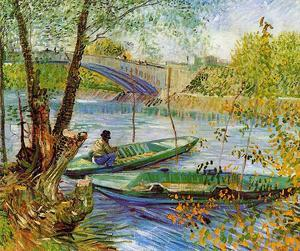
\includegraphics[width=0.3\textwidth]{interface/colour_histogram/colourvis1_o.jpg}
    }
    \subfigure[] {
                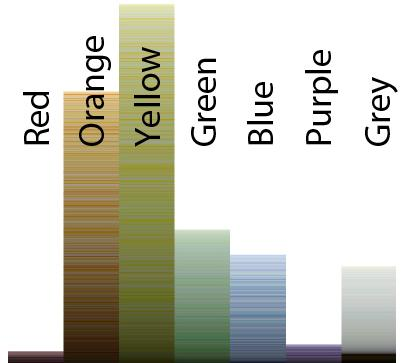
\includegraphics[width=0.3\textwidth]{interface/colour_histogram/colourvis1.jpg}
    }
  \caption{"Fishing in Spring, the Pont de Clichy" by Vincent van Gogh (a) and the corresponding labelled linear histogram representation.}
  \label{fig:colourvis1}
\end{figure}


\begin{figure}[htb]
	\centering
    \subfigure[] {
                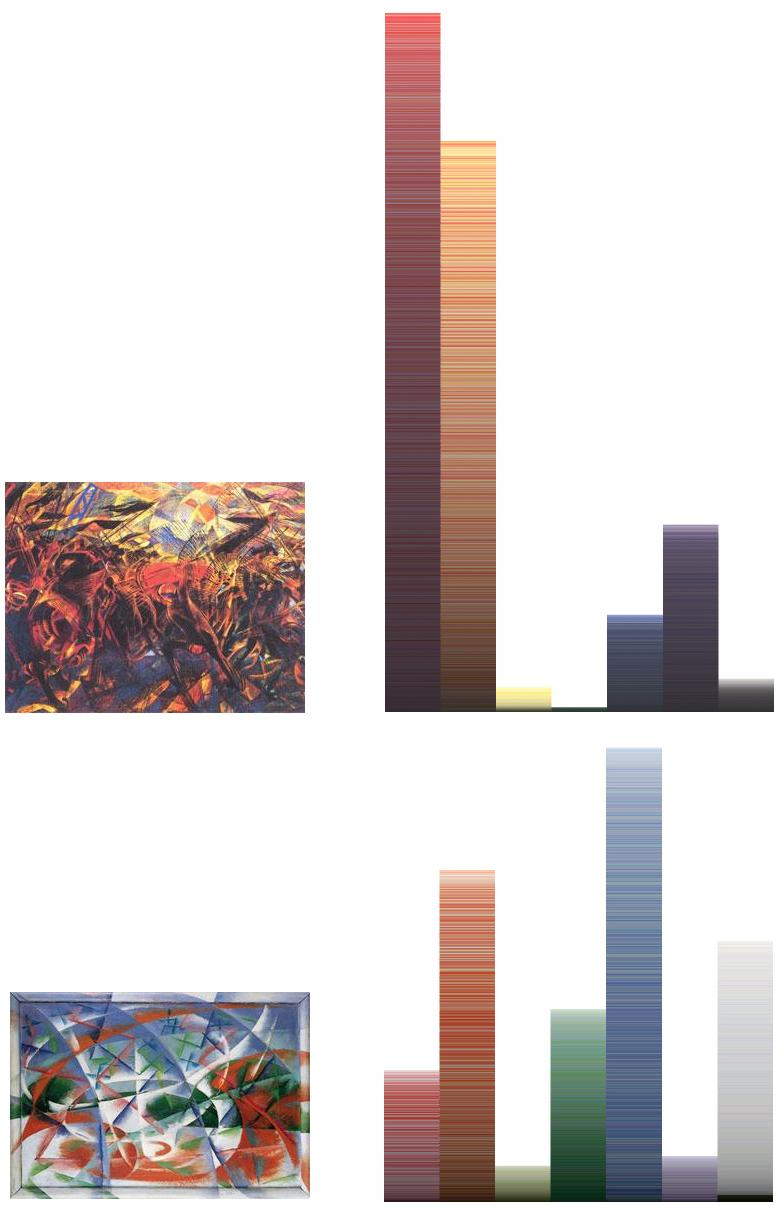
\includegraphics[width=0.3\textwidth]{interface/colour_histogram/colourvis2_o.jpg}
    }
    \subfigure[] {
                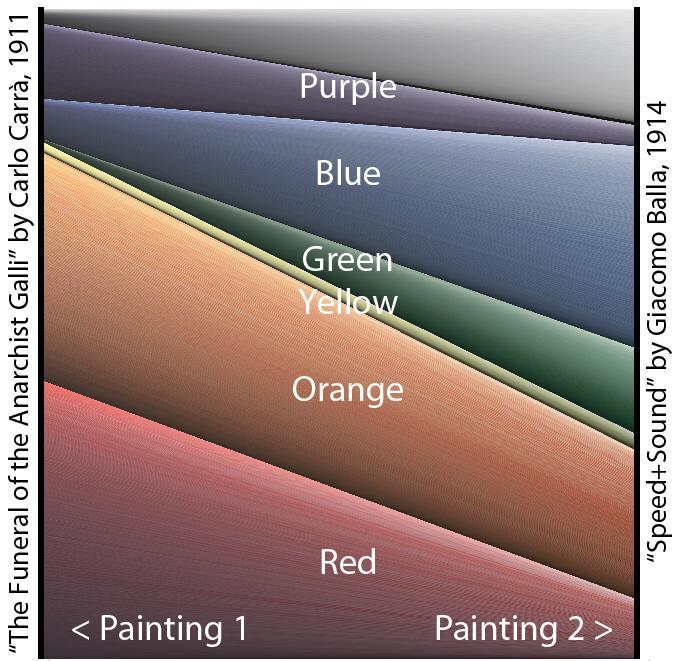
\includegraphics[width=0.4\textwidth]{interface/colour_histogram/colourvis2.jpg}
    }
  \caption{Linear histograms representations of “The Funeral of the Anarchist Galli” by Carlo Carrà (top) and “Speed+Sound” by Giacomo Balla (bottom) (a) with a labelled stacked line graph representation comparing the amount of each colour in both paintings (b).}
  \label{fig:colourvis2}
\end{figure}

Another important property is a colour saturation which is the colourfulness of a colour relative to its own brightness. The saturation of a colour is determined by a combination of light intensity and how much it is distributed across the spectrum of different wavelengths. The purest (most saturated) colour is achieved by using just one wavelength at a high intensity, such as in laser light. If the intensity drops, then as a result the saturation drops.

Colour saturation the influence the vividness of an image as a desaturated image is said to be dull, less colourful or washed out but can also make the impression of being softer. 


\subsubsection{Algorithm Description}

As described previously, colour is obviously a very important part in an image. With that being said, we implemented some simple algorithms that compute the amount of colour and saturation that exists in an image.

It was already said that an histogram is an important way to visualize the amount of each colour represented on the scenario. We also computed histograms to give this information. For our first implementation, we generated four histograms for each channel of the \emph{RGB} colour space and a grayscale version of the input image. Each frame to be processed comes in a packed format and is then converted both to a gray image and to a \emph{RGB} image. We then create a full-range histogram for each of the channels.

Knowing the amount of each colour in each one of the channels we can then obtain an interval that contains all the relevant colours. We considered as relevant colours, colours that have an amount of 5\% more than the maximum value. Since all histograms are normalized to a range of $[0,255]$, colours with a count higher than 12, are considered relevant. Given the colour range for each channel, we also calculate the amount of pixels that are near the limits. This amount is calculated by applying a Gaussian function where the peak is each one of the limits in the colour range. This can be translated by the equation
\begin{equation}
	\sum_{i \exists [0,50]}^{i}hist(i) + hist(i)*\frac{1}{0.7\sqrt{2\pi}}e^{-i},
	\label{eq:hist1}
\end{equation}
\begin{equation}
	\sum_{j \exists [205,255]}^{j}hist(j) + hist(j)*\frac{1}{0.7\sqrt{2\pi}}e^{-j}
	\label{eq:hist2}
\end{equation}
where the Gaussian function has the parameters $\sigma = 0.7, \sigma^{2} = 0.5$ and $\mu = 0$. $i$ and $j$ are the colour value in the histogram and $hist(i)$ is the amount of colour on the frame. The result from equations \ref{eq:hist1} and \ref{eq:hist2} are then used to represent visually the amount of pixels near each limit. 

In our second implementation we created another histogram but in this case we converted the input image to the \emph{HSV} colour space and performed an histogram over the \emph{Hue} channel. Due to the chosen method to visualize, the \emph{Hue} spectrum was quantized into six bins, which correspond to the primary colours red, green and blue, and its consequent secondary colours.
When processing the input image, a vector with a total length equal to the number of bins, would be accumulated depending on the colour of the pixel, since each bin covered a total of thirty colours with the \emph{Hue} spectrum. The amount percentage for each bin is then calculated and displayed to the user.

As mentioned in the previous section, the colourfulness of a scenario is always important considering that its what makes an image more vivid. Due to that fact, we also implemented a low saturation detector. This detector works by averaging the \emph{Saturation} channel in the \emph{HSV} colour space and compare its value to a threshold. If the value of saturation of an image is below a threshold of 50, then a suggestion is shown meaning that the use of a monochromatic filter might be useful in that situation. This threshold was defined by comparing the average saturation of 1000 images labelled as low-saturation images in the Flickr community.

\subsubsection{Interface Display}
In the previous section we described the algorithms for a saturation detector and two similar ways to calculate the colours presented in an image. For the later, it becomes even more important to correctly visualize that information.

For our first implementation which involved the calculation of three histograms based in the \emph{RGB} colour space and one with the image converted to gray scale, we tried to represent this information by using less space than a conventional histogram and by slightly simplifying the amount of information. As shown in Figure \ref{fig:hist_ex1}, our histograms are visualized by a bar with a dynamic size within certain limits which define the total range of colours within each channel. The purpose of this representation for the user to have a perception the amount of colours being used in each channel. The size of the bar is dynamic since it is defined by the first and last relevant colours found in a channel.

As mentioned before, this representation also shows the amount of pixels found near the boundaries of the colour range of each channel. This is represented by a line that grows vertically depending on the amount calculated by the equations \ref{eq:hist1} and \ref{eq:hist2}.

\begin{figure}[htb]
	\centering
    \subfigure[] {
                \includegraphics[width=0.45\textwidth]{interface/colour_histogram/ex1.png}
    }
    \subfigure[] {
                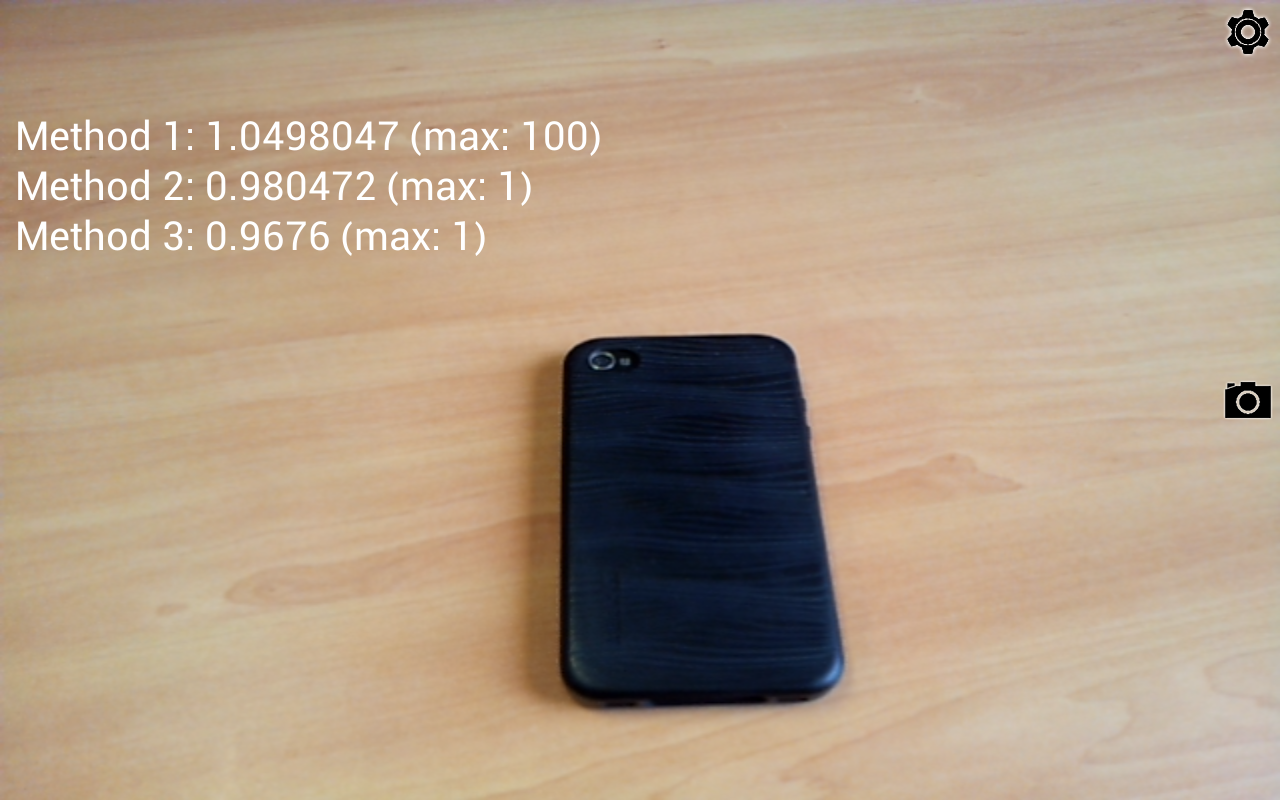
\includegraphics[width=0.35\textwidth]{interface/colour_histogram/ex1_2.png}
    }
  \caption{Visual cue chosen for the first implementation of the histogram being applied to a real-time scenario (a) and a reconstruction of the histogram made for the green channel that indicates de colour range in use and the amount of pixels near the limits (b).}
	\label{fig:hist_ex1}
\end{figure}

For the second implementation of an histogram, we chose to represent the \emph{Hue} concentration of each bin through a hexagon that resembles a colour wheel divided into six colours. Each section of the hexagon is filled with the percentage amount of the respective colour presented in the input image as shown in the Figure \ref{fig:hist_ex2}.

\begin{figure}[htb]
	\centering
    \subfigure[] {
                \includegraphics[width=0.45\textwidth]{interface/colour_histogram/ex2.png}
    }
    \subfigure[] {
                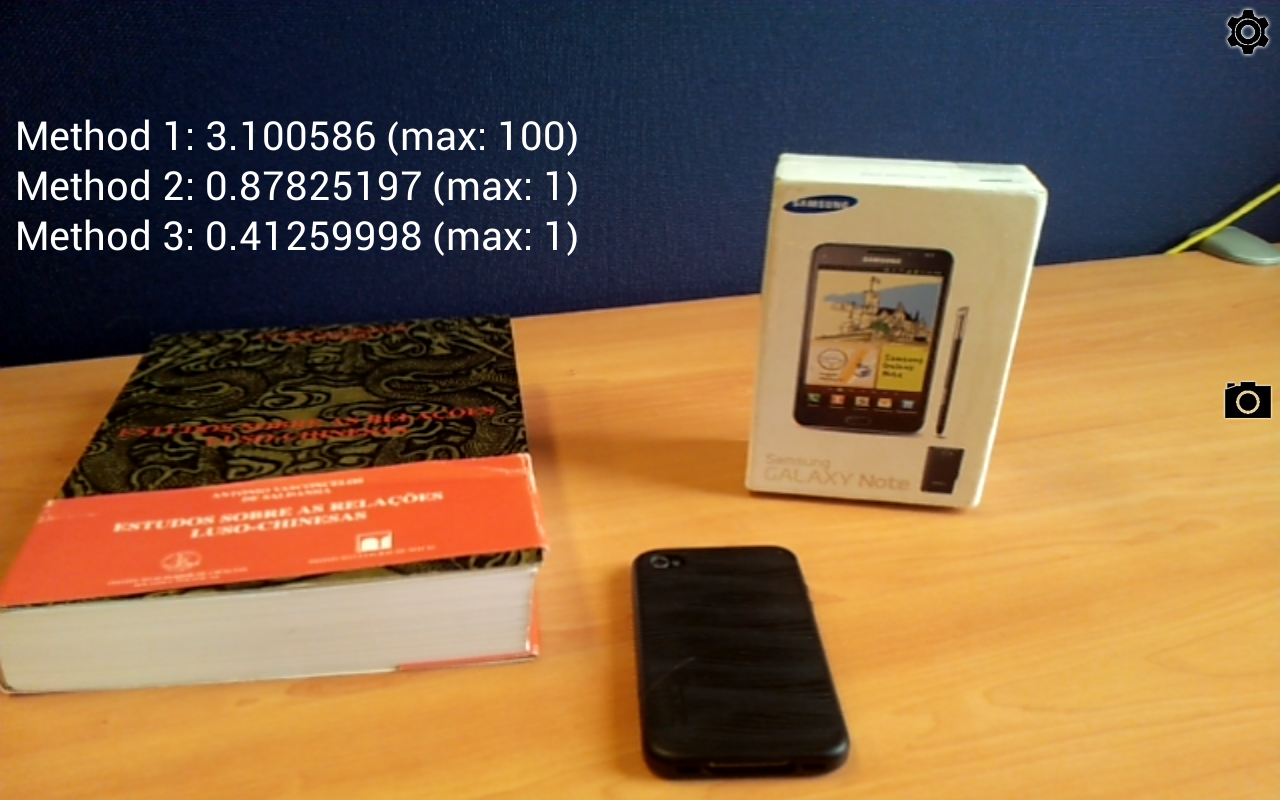
\includegraphics[width=0.35\textwidth]{interface/colour_histogram/ex2_2.png}
    }
  \caption{Visual cue chosen for the second implementation of the histogram being applied to a real-time scenario (a) and the resulting histogram isolated (b). }
	\label{fig:hist_ex2}
\end{figure}

For the saturation detection, we display a thumbnail with the real-time image converted into grayscale on the bottom-right corner of the viewfinder. This is an indicator that the usage of a monochromatic filter might be useful in that situation (Figure \ref{fig:hist_ex3}).

\begin{figure}[htb]
	\centering
	\includegraphics[width=0.45\textwidth]{interface/colour_histogram/ex3.png}
  	\caption{Frame detected as containing low saturation. Indicator shown on the bottom right corner highlighted in a red, which is the input frame converted into grayscale.}
	\label{fig:hist_ex3}
\end{figure}
  
\subsubsection{Discussion}
\label{subsub:disc_hist}
After implementing these features, we could conclude a couple of things. Starting by our first implementation of a histogram, the first noticeable problem is the fact that the histogram is made for the \emph{RGB} colour space. Although it is the most used colour space in image manipulation applications and photography systems, the conversion of real-world colours to \emph{RGB} is not direct.

With the representation we created a one-dimensional histogram that omitted the amount of each colour, to show a range of colours being used in the image. This range is determined by the first and last colours found as relevant with the purpose to show the spread of tones across a channel. As a general rule, in most cases a well balanced shot has a nice spread of tones which peak somewhere around the middle and taper off around the edges. Ignoring the peak around the middle and stabilization around the edges, we think this representation successfully serves the purpose giving an idea of the colours being used. The problem with this representation is that it does not contemplate any flaws in the middle of the histogram. This means that if it shows that a range of colours is being used, within that range, there's a possibility that some of the colours were not found in the image. Figure \ref{fig:disc_hist} illustrates this example. Imagining that the blue channel of an image as the histogram shown in Figure \ref{fig:disc_hist1}, there is a valley between two peaks that contains colours that weren't used. Figure \ref{fig:disc_hist2} displays our representation based on that histogram, where we can see that the concavity in the original histogram and the colours that were not used in that concavity, are shown as a part of the range of colours detected.

\begin{figure}[htb]
	\centering
    \subfigure[] {
                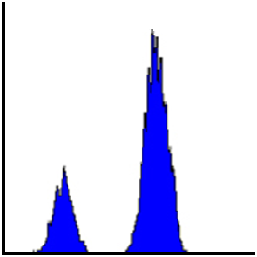
\includegraphics[width=0.3\textwidth]{interface/colour_histogram/hist1_ex.png}
                \label{fig:disc_hist1}
    }
    \subfigure[] {
                
\includegraphics[width=0.3\textwidth]{interface/colour_histogram/hist2_ex.png}
                \label{fig:disc_hist2}
    }
  	\caption{Illustrative figure of the problem found in our histogram representation (b) compared to the corresponding regular histogram (a).}
	\label{fig:disc_hist}
\end{figure}

Our second implementation uses an hexagon in resemblance of a colour wheel, it is easier to convert real-world colours to the \emph{HSV} colour space. Although it is easier to perceive the colours being used, it does not have into account the saturation or brightness of each colour. 
The main problem in this representation is the amount of percentages displayed. As it is, each part of the hexagon will be fully filled when all the \emph{Hue} values in the converted image are within the same range, which results in a scaling problem as this rarely happens. Each processed frame normally contains at least a small portion of all the colours presented in the wheel, meaning that with the representation chosen, small amounts of each section will be filled making them almost irrelevant. Even with this problem, the main purpose of this representation is to visualize the colours that have a higher presence in a scenario and what complementary colour should be used to provide a colour balance (Section \ref{subsub:colour_balance}).


As for our saturation detection method it is not very complex, however the threshold chosen to classify an input frame as highly saturated or not, was selected by averaging the saturation of 1000 images labelled as \emph{low saturation} by the Flickr's community. This being said the threshold was calculated over a set of static images which may have been digitally manipulated. This means that in a real-time scenario this threshold might not be the most appropriate as it is difficult to find scenarios to test and calculate a more adequate threshold. It would be necessary to find a large amount of real scenarios with low saturated colours and select manually filter them.

\subsection{Colour Templates and Hue Counting}
\label{sub:colour}

As said before, much of what viewers perceive and feel about a photo is through colours (Section \ref{subsub:colour_balance}). Although their colour perception depends on the context and is culture-related, colour science studies show that the influence on human emotions or feelings from a certain color or a certain color combination is usually stable under different culture backgrounds \cite{manav2007color}.
Professionals follow certain rules of color composition and scene composition to produce aesthetically pleasing photographs. For example, photographers focus on artistic color combination and properly put colour accents to create unique composition solutions and to invoke certain feelings among the viewers of their artworks. Therefore, exploring the relation between colours is a way to evoke those feelings.

\citeauthor{luo2008photo} explored the relation between colours \cite{luo2008photo}, in a feature to measure the color harmony of a photo in terms of learning the color combinations (coexistence of two colours in the photo) from the training dataset, to determine if a photo has a high or low quality.
For each photo in the dataset, a 50-bin histogram is generated for each channel in the \emph{HSV} colour space. The value of the color combination between hue $i$ and hue $j$ is defined as $H_{hue}(i) + H_{hue}(j)$, with a similar definition for the saturation and value channel. A histogram of high (low) quality training photos is generated by the formulas
\begin{equation}
H_{high,hue}(i,j) = Avg(H_{high,hue}(i)+H_{high,hue}(j)),
\end{equation}
\begin{equation}
H_{low,hue}(i,j) = Avg(H_{low,hue}(i)+H_{low,hue}(j)),
\end{equation}
with a similar process for combinations of $H_{high,sat}(i,j)$, $H_{low,sat}(i,j)$, $H_{high,sat}(i,j)$ and $H_{low,sat}(i,j)$.
To measure whether a photo is high or low quality based on the its colour combinations, the classifier is trained with the formula
\begin{equation}
f_{h} = Hue_{s}*Sat_{s}*Bri_{s},
\end{equation}
where $Hue_{s} = \frac{Hue_{high}}{Hue_{low}}$, $Sat_{s} = \frac{Sat_{high}}{Sat_{low}}$ and $Val_{s} = \frac{Val_{high}}{Val_{low}}$.
Although in \cite{luo2008photo}, the purpose of this feature is to train a classifier to identify the quality of a photo, it can also be used to query a database and obtain a set of images similar to the one being evaluated. Since our purpose with this thesis is to give useful information in real-time to the photographer, we explored the colour harmonization using the \emph{Hue} channel. Although we opted to not use any classifiers, we also implemented a score to each frame based on its hue count.

\subsubsection{Algorithm Description}
As mentioned before, we implemented a simple scoring system for each input frame and an algorithm that detects the harmonic colour template being used on a real-time input frame.

As for our scoring method, we implemented a feature described by \citeauthor{ke2006design} in \cite{ke2006design}, where the purpose is to measure its colour simplicity. One the main differences between professional photos and snapshots is that photos taken professionally are more colourful and vibrant depending on its brightness and saturation levels, while using a less number of unique hues. The first step in hue count is the conversion of the input frame to the \emph{HSV} colour space. After the colour space conversion, the \emph{Hue} channel is filtered by selecting pixels that have a brightness value in the range $[0.15,0.85]$ and saturation higher than 0.2 because the hue calculation would be inaccurate if otherwise. The next step is to calculate a 20-bin histogram $H$ with the hue values that passed the filter. After computing the histogram we select the number of bins $N$ that satisfy the equation

\begin{equation}
N = {i | H(i) > \alpha m},
\end{equation}
where $m$ is the maximum value of the histogram and $\alpha$ controls the noise sensitivity of the hue count. The author used $\alpha = 0.05$ as it produced good results for their training set. The final score is calculated by the equation
\begin{equation}
score = 20 - N.
\end{equation}

Our harmonic colour template detector is based in a method described in \cite{cohen2006color}. In the original article, the author uses a predetermined set of templates such as the ones in Figure \ref{fig:templates}, which can also be perceived as the colour distribution of the input image. The harmonic templates may consist of shades of the same colour (type $i, V, T$), complementary colours (type $I, Y, X$) or more complex combinations (type $L$). Although not used, the $N$-type template is applied to grayscale images. In our implementation we focused on templates for slight variations of the same colour and for complementary colours.

\begin{figure}[htb]
	\centering
	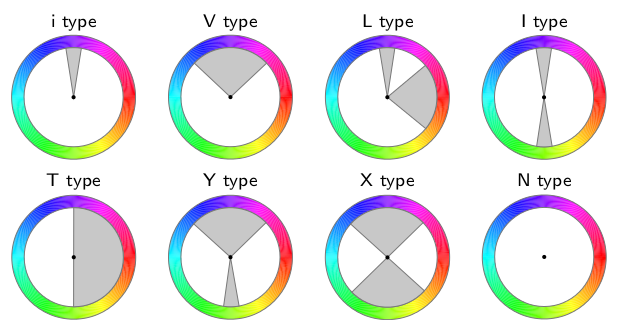
\includegraphics[width=0.5\textwidth]{interface/colour_template/templates.png}
  	\caption{Harmonic templates on the hue wheel. Colours that fall into gray areas are considered to be harmonic. Size and rotation of the gray areas may vary.}
	\label{fig:templates}
\end{figure}

The original article uses a hue histogram and tries to match the histogram with each of the templates in its various rotations. This method would prove to be computationally heavy on a mobile device in a real-time scenario, therefore, we opted to simplify the histogram and the template calculation. 

We started by converting the input image into the \emph{HSV} colour space and manipulate the \emph{Hue} channel. For our implementation, we used a wheel divided into twelve regions instead of using a full-colour wheel with enabled us to create a 12-bin histogram of quantized hues ordered by amount. The purpose of having an ordered histogram, is to obtain the first two main hues present in the image. Knowing the two main colours and its bins, we can map each bin into one region of a 360 degree wheel. This mapping is what will allow us to determine if a image fits into a monochromatic template or a complementary template, by calculating the difference between the bins of the two main colours.

After classifying an image as having a monochromatic or complementary template, starting in the most relevant bins, we verify if the adjacent bins have an occupation percentage in the image of at least 40\% of the starting bin. This will allow to know the size of template. Starting in a bin which is mapped into one region in the twelve-region colour wheel, we defined that the maximum size for a monochromatic template or one of the colours in a complementary template, is of three regions.

Since the scoring described before is based on a 20-bin histogram, we decided to modify it and perform the scoring based on a 12-bin histogram. This way, both the scoring and the template detection, are in accordance with one another.

\subsubsection{Interface Display}

For this feature, we chose to show colour wheel divided into twelve regions. This would prove to simplify both the implementation of the algorithm and display of the templates. Similarly to the original templates (Figure \ref{fig:templates}) the gray areas indicate the main colours present in the image and its neighbours that were considered relevant.
As for the scoring method, we took the most simple approach and decided to show the scoring result since both these methods are in accordance with one another.

\subsubsection{Discussion}

There are no major issues with each of these methods. However the most relevant issue, might be the size of templates. As mentioned before, starting in a bin we verify if the adjacent bins occupy a region that is at least larger than 40\% of the starting point, where the threshold was chosen experimentally with a dataset of static photographic images. The problem with choosing a threshold with a given dataset, is that the threshold might not work perfectly in a real-time scenario since the chance of getting snapshots while receiving real-time information is way higher then getting a frame that is considered to have aesthetic value.

\subsection{Face Detection and Composition Guidelines}
\label{sub:face_guidelines}

Since long, the detection and recognition of faces are areas of interest in the domain of computer vision. Such technology has been used in biometric identification, video-conferences and query systems.
Mobile devices are also able to find and recognize a face. Android provides a simple way to identify the faces of people in a bitmap image, with each face containing all the basic location information. Not just faces, but nowadays Android cameras already offer an API for detection of eyes and mouth and most recent versions are able to recognize faces to unlock such devices.

The fact that we can easily detect faces, enables us to explore some rules used in photography. One of these rules is the Rule of Thirds explained in Section \ref{subsub:rule_thirds} which states that for an image to be visually interesting, the main focus of the image needs to lie along one of the lines marked in thirds, or the intersection points between those lines\cite{kamps2012rules}.

Other rule is the Rule of Odds which states that images are more visually appealing when there is an odd number of subjects. For example, if we are going to place more than one person in a photograph, we should use 3 or 5 or 7, etc \cite{kamps2012rules}. Studies have shown that people are actually more at ease and comfort when viewing imagery with an odd number of subjects. This rule can also be boosted by using triangles, since a triangle is one of the strongest compositional shapes, as it can add a sense of visual unity. In essence, a triangle is a closed curve incorporating at least one diagonal. Since the curve is closed, it won't lead the eye outside of the frame. A single triangle in in the middle of the frame can lead to a somewhat static composition, but triangular composition can be found in many famous works of art.

By combining these rules with a facial detection system, we devised a feature that could be helpful in respecting these essential guideline in photography composition.

\subsubsection{Algorithm Description}

For this feature we tried to mix the rules previously stated with face detection in a real-time environment. Although it can be used separately, we implemented the two simple grids that follow the Rule of Thirds (Section \ref{subsub:rule_thirds}) and the Rule of the Golden Section (Section \ref{subsub:golden_section}) that uses the golden ratio.

As far as implementing these grids, there was no difficulty since it was only needed to obtain the device screen size and generate four lines for each rule, where these lines would divide the screen in 9 equal parts for the Rule of Thirds or in in sections with a proportion of 1.6:1 as shown in Figure \ref{fig:golden_section2}.

These guideline would then be useful to test different compositions with faces detected. As for detection of faces, we opted by using the mechanisms available in \emph{OpenCV} instead of using the ones available by Androids API. This is due to the fact that our objective was of creating a library to run only in JNI. If we opted by using the Androids API, then it would become specific of the application instead of being portable code for other application.
With the \emph{OpenCV} library we used the Haar feature-based classifier to detect faces \cite{viola2001rapid}. This method needs a big set of positive and negative images to train the classifier. This train is based on the extraction of haar features, as the ones shown in Figure \ref{fig:haar_features}. After training a classifier, the implemented algorithm uses the concept of Cascade of Classifiers where a total of 6000 features are divided by groups of features, and for a small window in an image the first group of features is tested. If that region is a non-face region, it is forever discarded and passes to the next group of features that can then concentrate on testing the remaining regions where there's a probability of finding a face. The regions where the faces are found, are then returned and used by us.

Having detected the faces position and the lines for the grids, we can the calculate the distance between the center of a face region and the nearest intersection line. The intersection with the smallest distance, is the most viable placement for the subject in accordance to the Rule of Thirds.

\begin{figure}[htb]
	\centering
	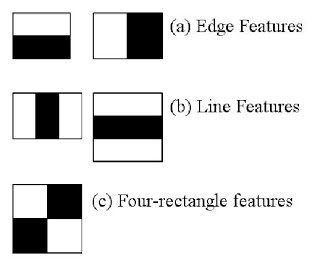
\includegraphics[width=0.4\textwidth]{interface/face/haar_features.jpg}
  	\caption{Type of convolution kernels used to extract features \cite{OCV}.}
	\label{fig:haar_features}
\end{figure}

\subsubsection{Interface Display}

We started by describing the Rule of Thirds and Rule of Golden Section that are viewed as a simple grid over the viewfinder that respects the proportions established by both rules, as illustrated by Figure \ref{fig:face_ex1} and Figure \ref{fig:face_ex2}.
As for the detection of faces, we took the most common approach. Since we know the position of the regions that contain faces, we opted to draw a bounding rectangle around that regions (Figure \ref{fig:face_ex3}, \ref{fig:face_ex3}).

After detecting faces we test to see if there are three faces detected. This is so that we can apply the concept of the Rule of Odds with the detected faces. If there are three faces then we can also try and boost the composition by linking their positions and form a triangle. We display the connection between the faces by drawing lines between them.

Figure \ref{fig:face_ex4} illustrates this triangle formed by the detected faces as well as the suggestions. Each of the intersection points on both grid highlights when it is a suggested point for a face. To complement the triangle composition when three faces are detected, we also suggest a triangular composition with the nearest intersection points of the grid in cyan blue as shown in Figure \ref{fig:face_ex5} and Figure \ref{fig:face_ex6}.
\begin{figure}[htbp]
	\centering
    \subfigure[] {
                \includegraphics[width=0.45\textwidth]{interface/face/ex1.png}
                \label{fig:face_ex1}
    }
    \subfigure[] {
                \includegraphics[width=0.45\textwidth]{interface/face/ex2.png}
                \label{fig:face_ex2}
    }
    \subfigure[] {
                \includegraphics[width=0.45\textwidth]{interface/face/ex3.png}
                \label{fig:face_ex3}
    }
    \subfigure[] {
                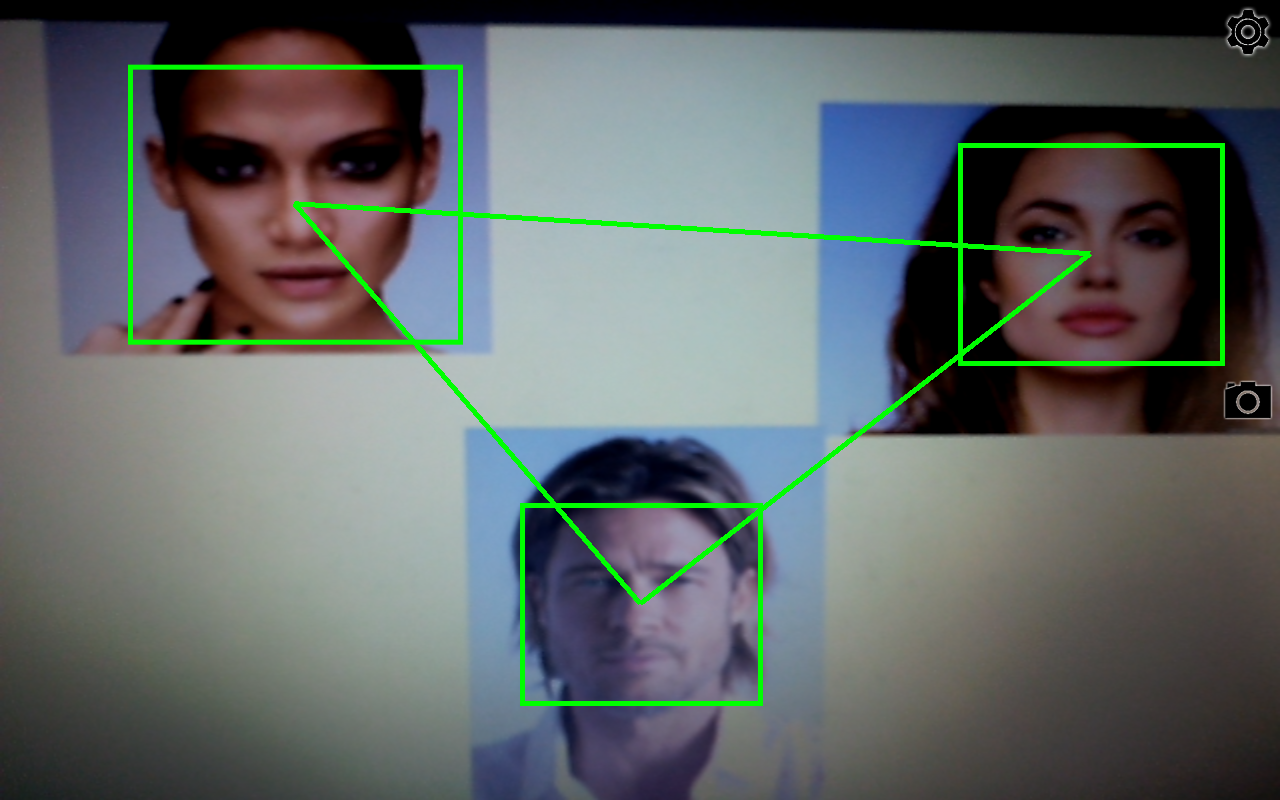
\includegraphics[width=0.45\textwidth]{interface/face/ex4.png}
                \label{fig:face_ex4}
    }
    \subfigure[] {
                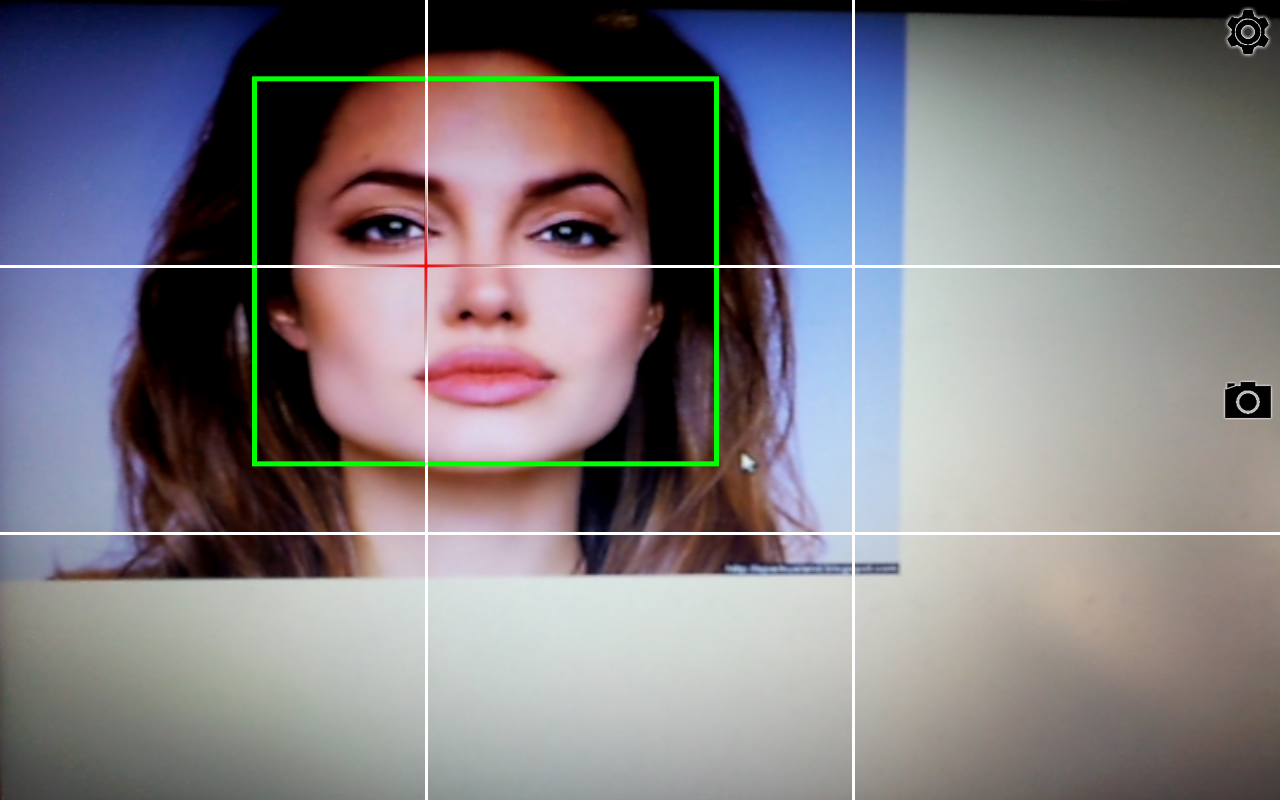
\includegraphics[width=0.45\textwidth]{interface/face/ex5.png}
                \label{fig:face_ex5}
    }
    \subfigure[] {
                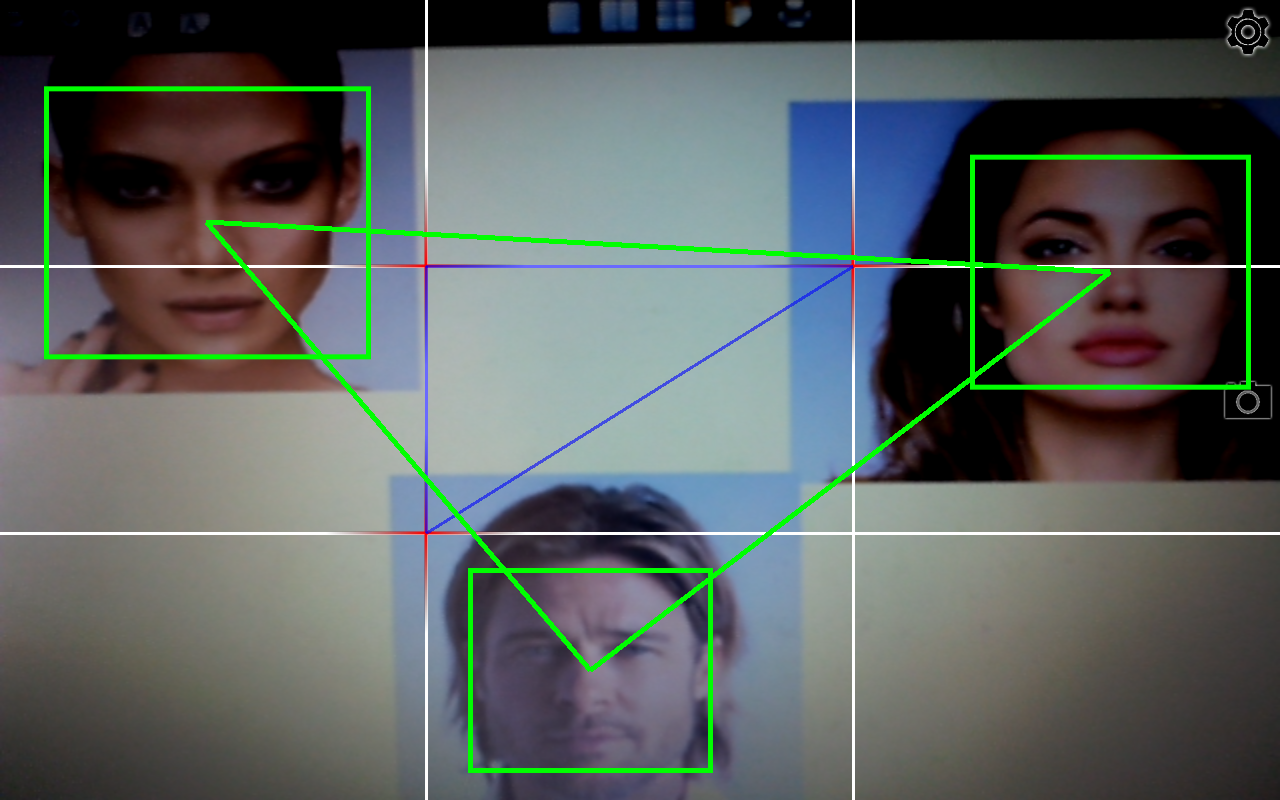
\includegraphics[width=0.45\textwidth]{interface/face/ex6.png}
                \label{fig:face_ex6}
    }
  	\caption{Multiple visual cues used to implement this features, such as helping grid (a,b), face detection (c,d) and a mixture of both (e,f), tested when detecting one or three faces.}
	\label{fig:face_interface}
\end{figure}

\subsubsection{Discussion}

Due to the simple implementation, there aren't any particular problems. The face detection might be the most prone to problems part. As referred before, the face detection uses a trained classifier and we used a default classifier for frontal face recognition provided by the \emph{OpenCV} library. Therefore, this classifier will not detect faces in profile.

Although the user can choose which feature to display at a time, when they are all activated, this many visual cues are quite distracting and occupy a lot of space in the interface.

However, as a proof of concept this visual cues do work but its important to keep in mind that the positions suggested, are simple suggestions, as it is not a recipe for obtaining aesthetic results. The user must always have the final word for the placement of the detected faces, on the importance of having odd number of elements and on the exploration of triangular compositions.

\subsection{Object Segmentation}
\label{sub:segmentation}

Unless it is a photography of a seascape or a landscape, it is normal for a photo to have a relevant subject. With this in mind, segmentation of a subject in multiple scenarios might be useful to attain a better composition.

Segmentation of an object in a photo, is a topic that has already been widely researched. One of the simplest ways of extracting information about the object in a real-time scenario is to have information about its background beforehand and subtract it. 

\citeauthor{yang2004real} \cite{yang2004real} describe a system for security cameras, able to recognize and track a moving object. This is possible once the system is collecting information about the background as time passes. Using the information about the background, the system can subtract any object that considers strange to the background, and start the tracking. This method has the advantage of being fast and discards the possibility of training a classifier for object identification. 
\citeauthor{butler2003real} describe a similar approach \cite{butler2003real}, where the key is to learn the background and generate a model of it by representing each pixel in the frame by a group of clusters, where these clusters are ordered by the likelihood of modelling the background. Incoming pixels are matched against the corresponding cluster group and classified as part of the background.
In our case, these methods have an obvious problem. Normally, the subject is already placed when the user wants to take a photo, therefore, the subject would be confused as a background or, the user would have to point the camera before placing the subject to initiate a process of extracting information and learn what is the background. When talking about a  camera in a mobile device or any digital camera, this method is nearly impractical, as the regular user tends to move the arms quite easily ruining the learning process started before. Thus, being an unreliable method for object segmentation.

For our use case, we envision a method for generic object segmentation that could be used in real-time. Since it is for generic objects, we couldn't train a classifier to recognize multiple objects, or use edges information for comparison, as it would need multiple photos for data collection, and the segmentation would be limited to a few objects. 

\subsubsection{Algorithm Description}
\label{subsub:seg_algorithm}

Colour is a very important feature in a photo \cite{kamps2012rules, Santos}. With this in mind, when photographing, the main subject should cause visual impact due to its contrast relative to the background or other elements in the scenery. For this, we used a slightly simplified version of the \emph{Histogram Based Contrast} (HC) method described by \citeauthor{cheng2011global} in \cite{cheng2011global} for extraction of salient regions in a photo that evaluates global contrast differences, calculating saliency values for image pixels using colour statistics. The saliency of a pixel is defined using its colour contrast to all other pixels in the image. This can be described as,

\begin{equation}
S(I_{k}) = \sum_{\forall I_{i} \in I} D(I_{k}, I_{i}),
\end{equation}

where $D(I_{k}, I_{i})$ is the colour distance between saliency value $I_{k}$ and pixel $I_{i}$ in the input image in the \emph{L*a*b*} colour space. Since this is computationally expensive, \citeauthor{cheng2011global}, reduces the number of colours needed to consider, by quantizing each colour channel to have 12 different values, reducing the number of colours to $12^{3} = 1728$. Since a natural image covers only a small portion of the full colour space, the less occurring colours are ignored, ensuring that the most occurring ones, cover at least 95\% of the image pixels. The remaining 5\% are replaced by the closest colours in the histogram. Since this quantization might introduce artifacts, the author preforms a smoothing procedure over each saliency value. Each saliency value is replaced by the weighted average of the $n/4$ neighbours where $n$ is the number of colours that fill 95\% of the image pixels.

After obtaining a saliency map, the map is turned into a binary segmentation mask using a fixed threshold. Finally GrabCut \cite{rother2004grabcut} will be used repeatedly to refine the segmentation result initially obtained by the binary segmentation mask.

\subsubsection{Implementation Details}

To use this algorithm in a real-time scenario in a mobile device, our implementation had to be simplified. GrabCut is too heavy to run smoothly on a mobile device, and for that reason, we had to discard its usage sacrificing the refinement of the segmentation for speed. After obtaining the saliency map described in \cite{cheng2011global}, we give a label to each pixel depending on its value. These labels would be used in GrabCut to define which pixels are considered foreground, probable foreground, background, or probable background. In our case, we used the labels to create masks with the areas defined as probable foreground and probable background. A pixel is classified as probable foreground if its value was larger or equal to 200 and probable background if it was between 20 and 200. We defined experimentally the thresholds using images from the dataset used to test the original algorithm.

After obtaining a mask with each pixel labelled, we created a mask with all pixels that were considered as probable foreground and calculated the center of mass for the resulting mask. To remove artifacts that might exist from using an incorrect threshold value, we generate a bounding rectangle that starts at the calculated center of mass and expands in every direction. Each edge will continue expanding while each row or column that passes, has at least a count of 25 pixels belonging to the segmentation mask, and stops when 50 rows or columns have been covered with a count of pixels bellow the previously stated. These thresholds were found experimentally and seem reasonable for the test images.

The obtained bounding rectangle and mask with areas considered probable foreground, is a good estimate of what was the main object in the scenario. The result of the segmentation was a section of the mask containing the probable foreground pixels, cropped in the area defined by the bounding rectangle. Since this algorithm is not sensitive to slight variations in lightning, we merged the probable foreground pixels with the probable background ones and cropped with the bounding rectangle. This would later be helpful filling the gaps in the mask, as this algorithm was not sensitive to slight light changes.

\subsubsection{Interface Display}

After generating the mask we chose to simply show a semi-transparent mask over the live feed obtained from the camera, as shown in Figure \ref{fig:interface_segmentation}. This would be a good indicator of what is the subject in the scenario and if it had any colour striking features relatively to the rest of the elements.

\begin{figure}[htbp]
	\centering
	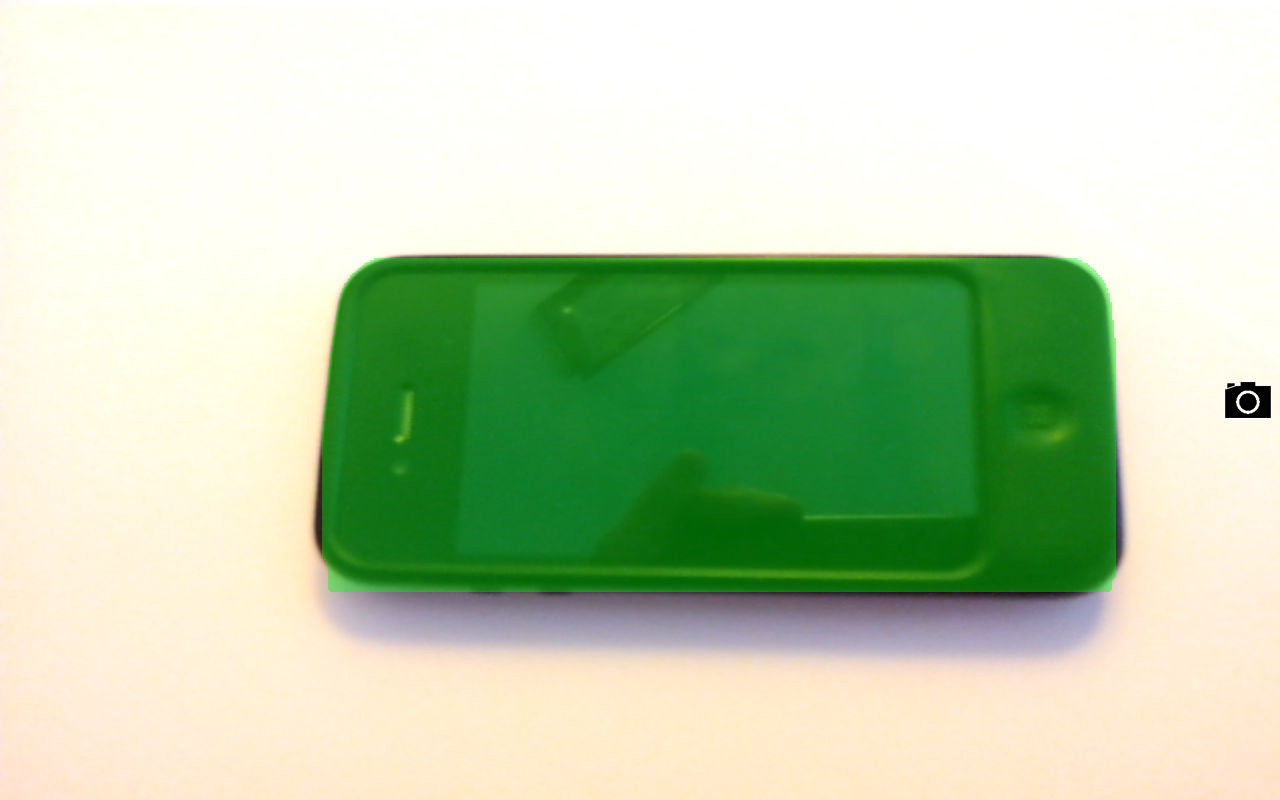
\includegraphics[scale=0.2]{interface/interface_segmentation.png}
    \caption{Example of object segmentation interface. The resulting mask of the algorithm is then displayed as a green overlay in the camera live feed.}
  	\label{fig:interface_segmentation}
\end{figure}

This could also be used together with a guideline such as Rule of Thirds, described in Section \ref{sub:face_guidelines}, to reposition the object and change the composition.

\subsubsection{Discussion}
\label{subsub:seg_discussion}
Being a simplified version of the original algorithm, it does not work perfectly. Since it depends on the global contrast of a subjects colours, this segmentation might not work if the background is not plain or simple. Figure \ref{fig:seg_example} show the multiple stages taken to segment an object in an image and its final result.
\begin{figure}[htb]
	\hspace*{-45pt}
    \begin{tabular}{cccccccc}
    	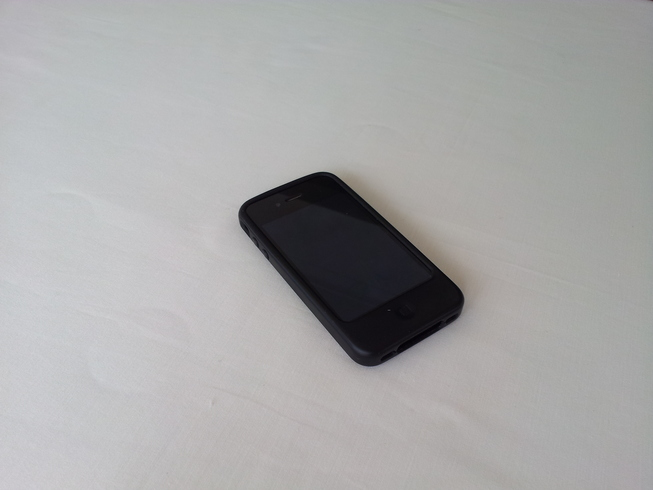
\includegraphics[width=0.14\textwidth]{interface/segmentation/3/re_3.jpg}        &
		\hspace*{-13pt}    	
    	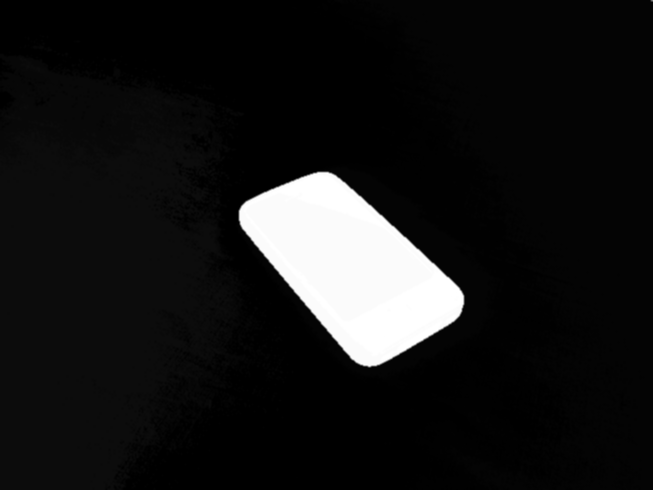
\includegraphics[width=0.14\textwidth]{interface/segmentation/3/re_3_sal.png}    & 						\hspace*{-13pt}
    	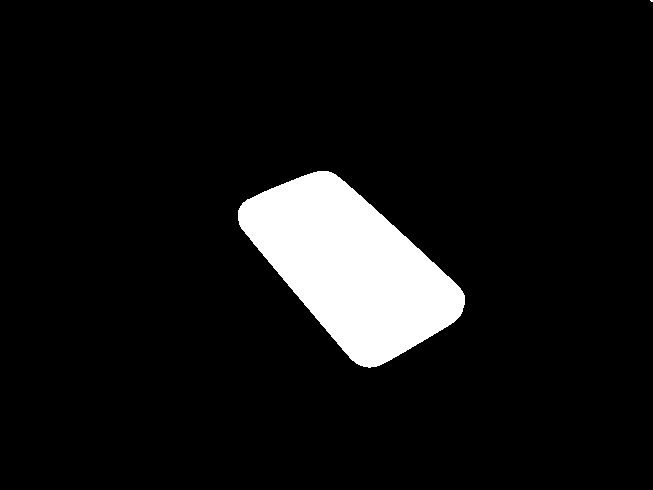
\includegraphics[width=0.14\textwidth]{interface/segmentation/3/re_3_bmask.png}    & 					\hspace*{-13pt}
    	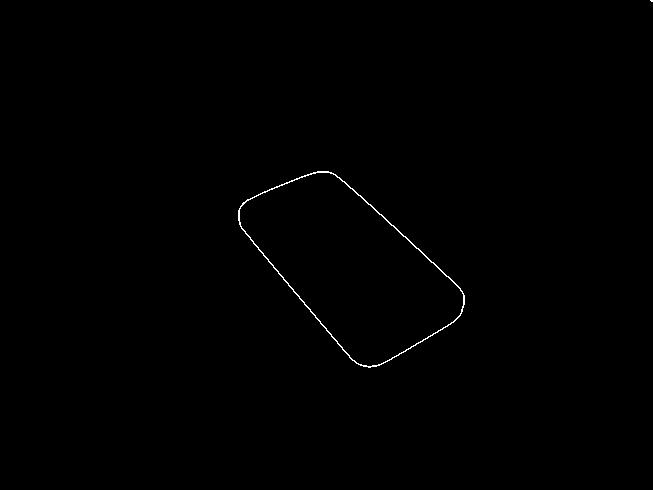
\includegraphics[width=0.14\textwidth]{interface/segmentation/3/re_3_pr_bgd.png}    & 					\hspace*{-13pt}
		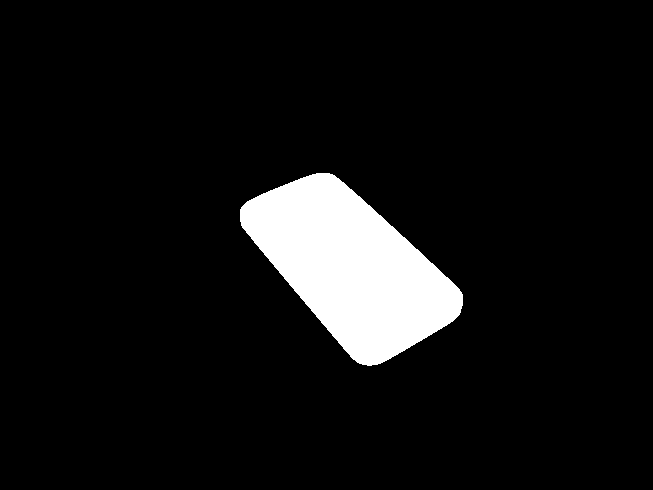
\includegraphics[width=0.14\textwidth]{interface/segmentation/3/re_3_pr_fgd.png}    & 					\hspace*{-13pt}
		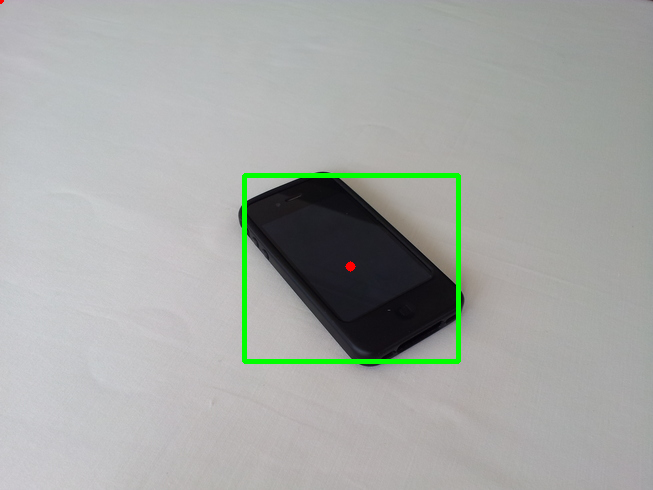
\includegraphics[width=0.14\textwidth]{interface/segmentation/3/re_3_rect.png}    & 					\hspace*{-13pt}
		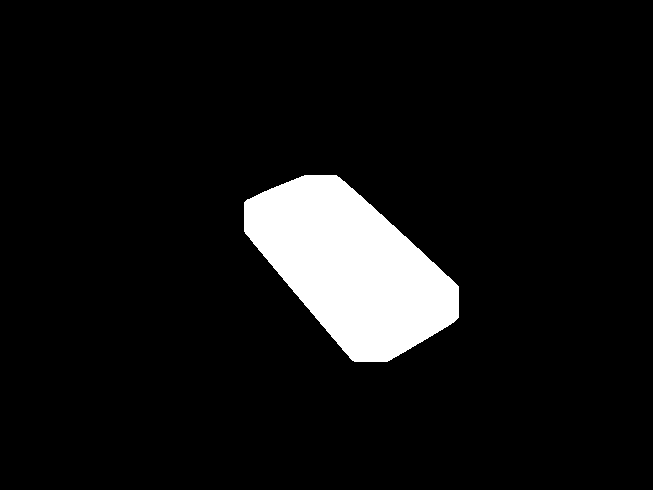
\includegraphics[width=0.14\textwidth]{interface/segmentation/3/re_3_mask.png}    & 					\hspace*{-13pt}
		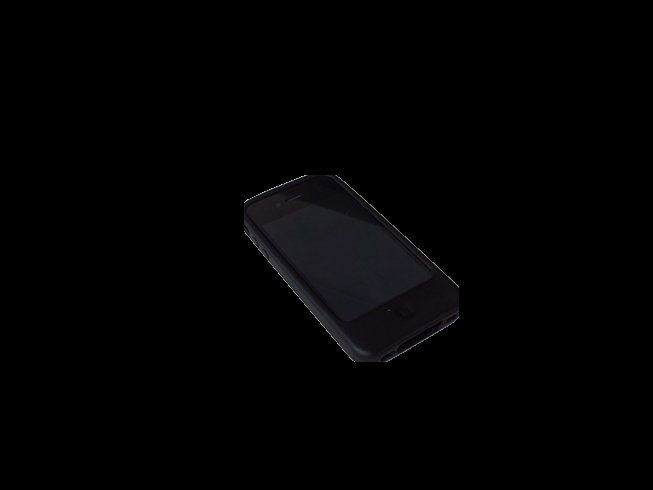
\includegraphics[width=0.14\textwidth]{interface/segmentation/3/re_3_seg.png} \\
    
    	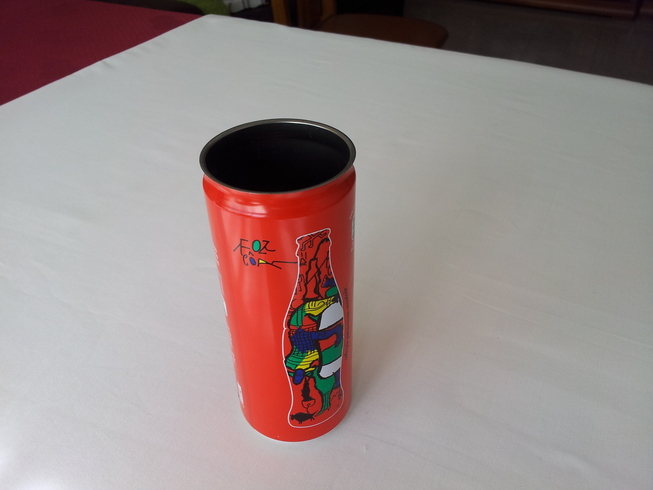
\includegraphics[width=0.14\textwidth]{interface/segmentation/2/re_2.jpg}    & 							\hspace*{-13pt}
		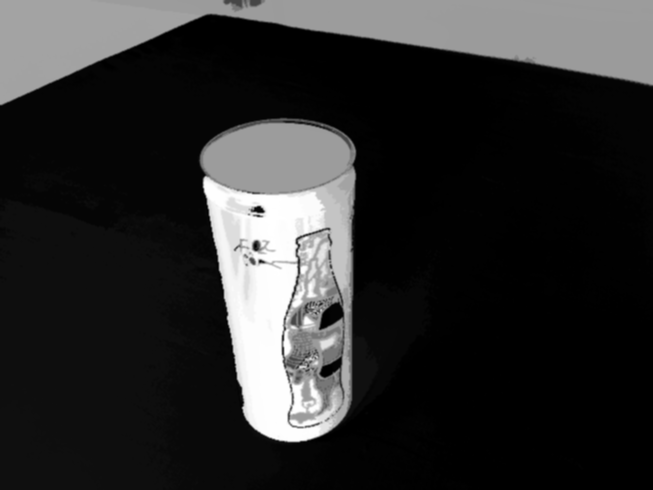
\includegraphics[width=0.14\textwidth]{interface/segmentation/2/re_2_sal.png}    & 						\hspace*{-13pt}
		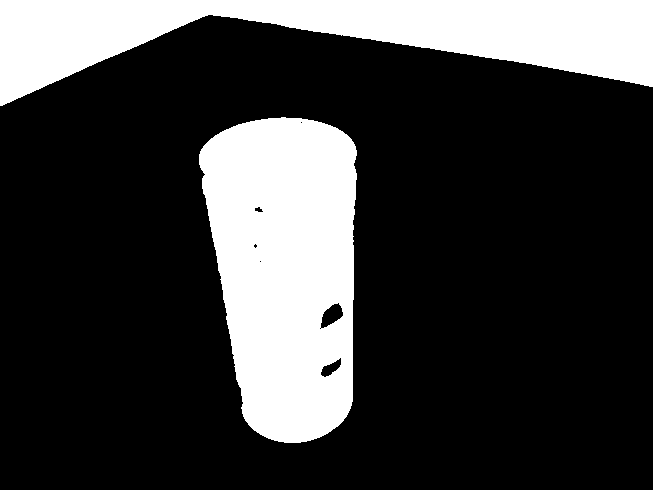
\includegraphics[width=0.14\textwidth]{interface/segmentation/2/re_2_bmask.png}    & 					\hspace*{-13pt}
		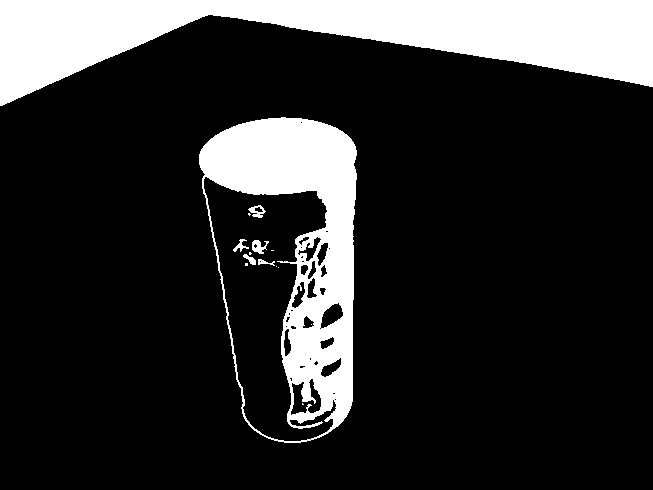
\includegraphics[width=0.14\textwidth]{interface/segmentation/2/re_2_pr_bgd.png}    & 					\hspace*{-13pt}
		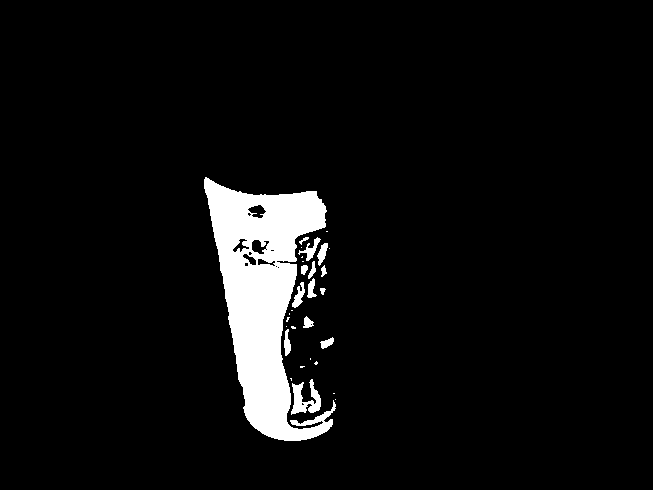
\includegraphics[width=0.14\textwidth]{interface/segmentation/2/re_2_pr_fgd.png}    & 					\hspace*{-13pt}
		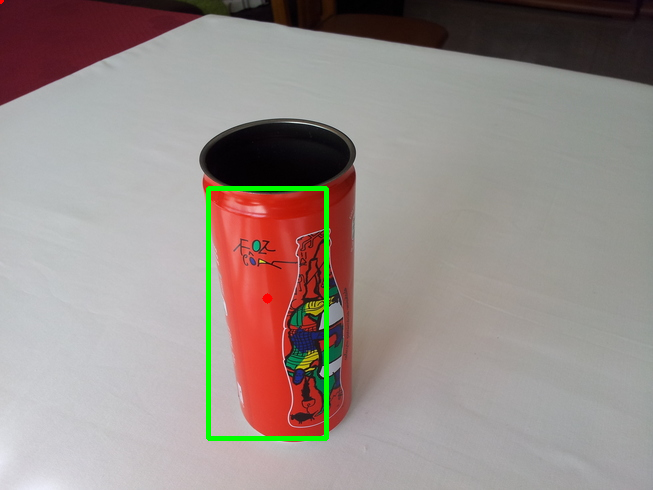
\includegraphics[width=0.14\textwidth]{interface/segmentation/2/re_2_rect.png}    & 					\hspace*{-13pt}
		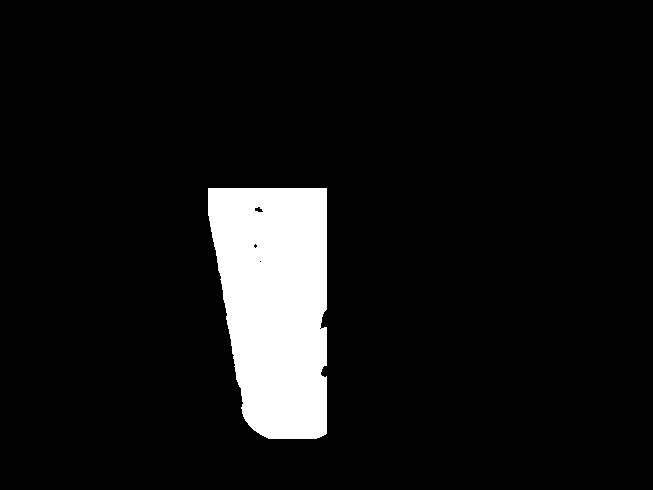
\includegraphics[width=0.14\textwidth]{interface/segmentation/2/re_2_mask.png}    & 					\hspace*{-13pt}
		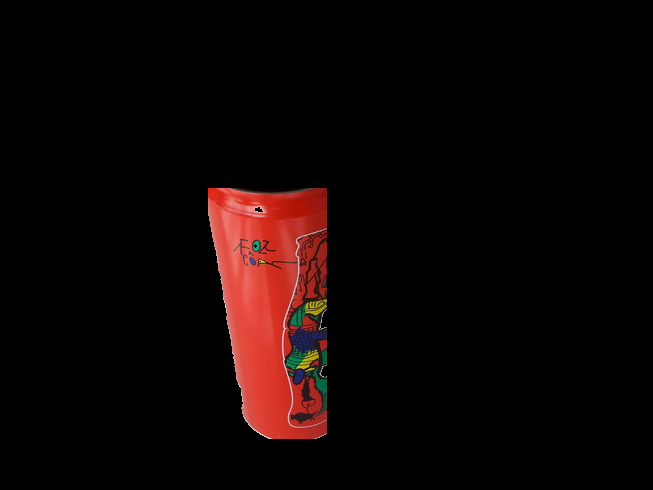
\includegraphics[width=0.14\textwidth]{interface/segmentation/2/re_2_seg.png} \\
                
    	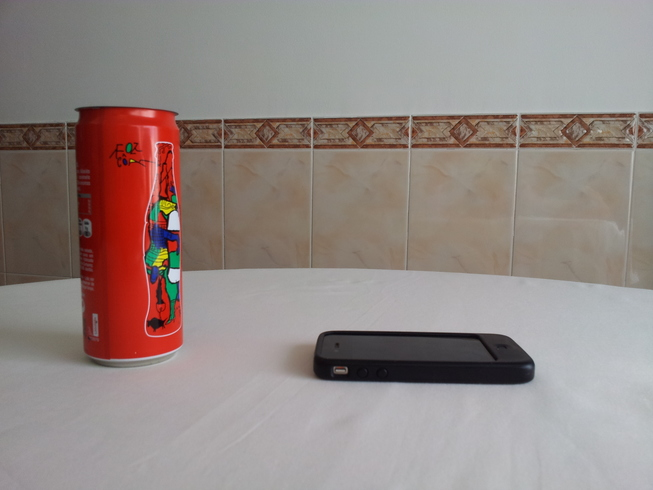
\includegraphics[width=0.14\textwidth]{interface/segmentation/4/re_4.jpg}    & 							\hspace*{-13pt}
		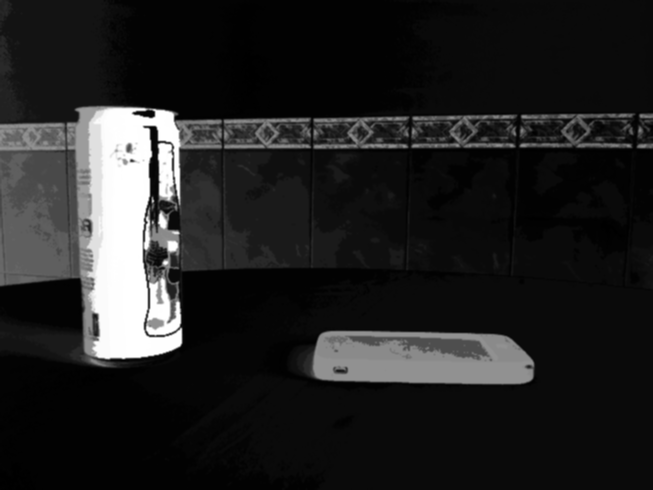
\includegraphics[width=0.14\textwidth]{interface/segmentation/4/re_4_sal.png}    & 						\hspace*{-13pt}
		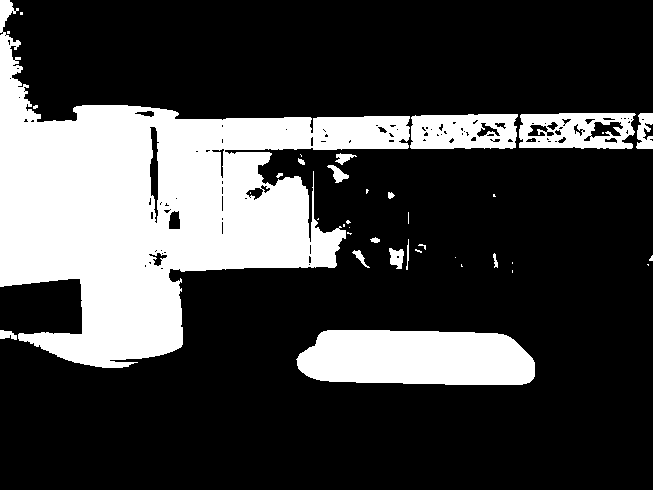
\includegraphics[width=0.14\textwidth]{interface/segmentation/4/re_4_bmask.png}    & 					\hspace*{-13pt}
		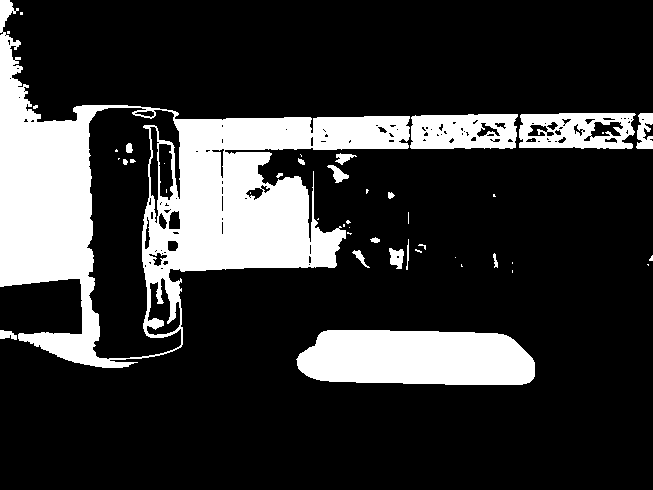
\includegraphics[width=0.14\textwidth]{interface/segmentation/4/re_4_pr_bgd.png}    & 					\hspace*{-13pt}
		
\includegraphics[width=0.14\textwidth]{interface/segmentation/4/re_4_pr_fgd.png}    & 					\hspace*{-13pt}
		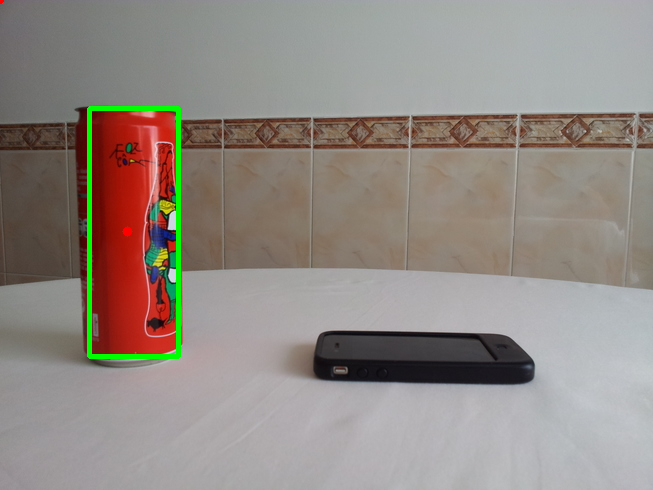
\includegraphics[width=0.14\textwidth]{interface/segmentation/4/re_4_rect.png}    & 					\hspace*{-13pt}
		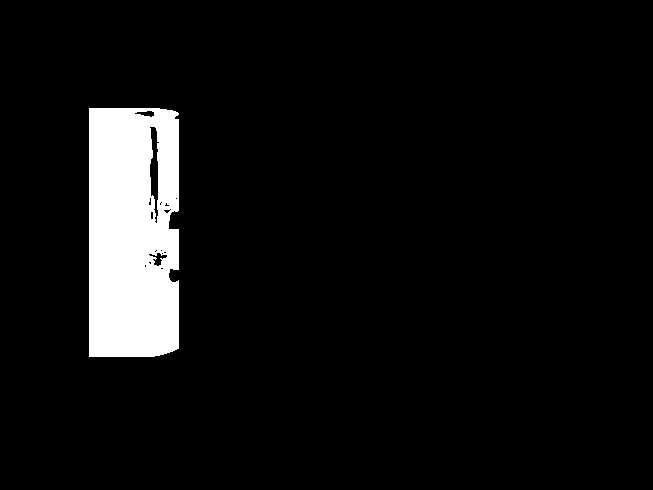
\includegraphics[width=0.14\textwidth]{interface/segmentation/4/re_4_mask.png}    & 					\hspace*{-13pt}
		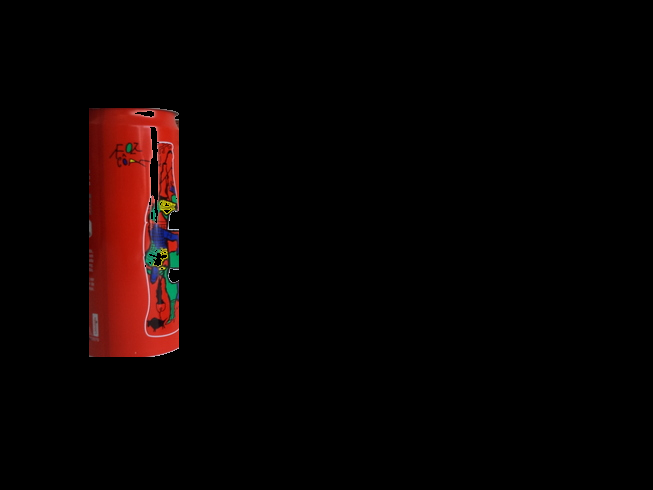
\includegraphics[width=0.14\textwidth]{interface/segmentation/4/re_4_seg.png} \\
		
		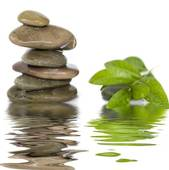
\includegraphics[width=0.14\textwidth]{interface/segmentation/10/10.jpg}        &
        \hspace*{-13pt}
		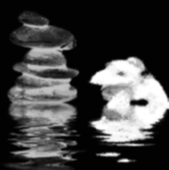
\includegraphics[width=0.14\textwidth]{interface/segmentation/10/10_sal.png}    & 						\hspace*{-13pt}		
		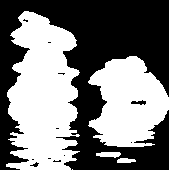
\includegraphics[width=0.14\textwidth]{interface/segmentation/10/10_bmask.png}    & 					\hspace*{-13pt}		
		\includegraphics[width=0.14\textwidth]{interface/segmentation/10/10_pr_bgd.png}    & 					\hspace*{-13pt}		
		\includegraphics[width=0.14\textwidth]{interface/segmentation/10/10_pr_fgd.png}    & 					\hspace*{-13pt}		
		\includegraphics[width=0.14\textwidth]{interface/segmentation/10/10_rect.png}    & 						\hspace*{-13pt}		
		\includegraphics[width=0.14\textwidth]{interface/segmentation/10/10_mask.png}    &
		\hspace*{-13pt}		
		\includegraphics[width=0.14\textwidth]{interface/segmentation/10/10_seg.png} \\
		
		\includegraphics[width=0.14\textwidth]{interface/segmentation/7/re_7.jpg}        &
        \hspace*{-13pt}
		\includegraphics[width=0.14\textwidth]{interface/segmentation/7/re_7_sal.png}    & 						\hspace*{-13pt}		
		\includegraphics[width=0.14\textwidth]{interface/segmentation/7/re_7_bmask.png}    & 					\hspace*{-13pt}		
		\includegraphics[width=0.14\textwidth]{interface/segmentation/7/re_7_pr_bgd.png}    & 					\hspace*{-13pt}		
		\includegraphics[width=0.14\textwidth]{interface/segmentation/7/re_7_pr_fgd.png}    & 					\hspace*{-13pt}		
		\includegraphics[width=0.14\textwidth]{interface/segmentation/7/re_7_mask.png}    & 					\hspace*{-13pt}		
		\includegraphics[width=0.14\textwidth]{interface/segmentation/7/re_7_rect.png}    &
		\hspace*{-13pt}		
		\includegraphics[width=0.14\textwidth]{interface/segmentation/7/re_7_seg.png} \\
		a) & \hspace*{-13pt} b) & \hspace*{-13pt} c) & \hspace*{-13pt} d) & \hspace*{-13pt} e) & \hspace*{-13pt} f) & \hspace*{-13pt} g) & \hspace*{-13pt} h)
    \end{tabular}
    \caption{Steps taken when segmenting an object. a) Input image. b) Saliency map generated by the algorithm in \cite{cheng2011global}. c) Binary mask. d) Probable background pixels. e) Probable foreground pixels. f) Bounding rectangle and center of mass point. g) Cropped mask containing the probable foreground area filled in with probable background pixels. h) Segmentation applied to the input image.}
    
	\label{fig:seg_example}	      
\end{figure}

As it is possible to observe in Figure \ref{fig:seg_example}, the input image shows a singular object in a plain background with a successful segmentation. In the second image it is possible to confirm that, although the object is detected, the foreground threshold is not sensitive to lightning changes, as the darkest side in the can is considered as being a probable background.

This algorithm also might not work when trying to segment two objects. Example of this is the third input image in Figure \ref{fig:seg_example}, where we can verify by the saliency map, that the can is obviously more salient than the other object, therefore the second object is classified as probable background. Another example of this is the fourth image. With a plain background and two objects, the object with more vivid colours is the one considered as foreground, leaving the remaining object as part of the foreground.

The fifth image shows an example were lightning changes affect the outcome of the algorithm. In this case, the can and a part of the wall are considered as foreground. The solution to this would be a higher threshold when defining the foreground pixels, as the wall is visibly less salient than the can in the saliency map. Since it is detecting the wall as a part of the foreground, this causes the center of mass to be slightly dislocated and generates a larger bounding rectangle. When merging the probable foreground pixels with the probable background ones and cropping with the bounding rectangle, it segments a big portion of the image that its not relevant.

This object segmentation method was also used in other functionalities implemented for this thesis.

\subsection{Image Simplicity}
\label{sub:background}

To reduce the attention distraction by the objects in the background, photographers usually make the background simple. With that perspective in mind, the simplicity of a photo was considered a good feature to analyse.
The most easiest form to obtain simplicity is to place the subject against a neutral background like a backdrop or the sky. Backgrounds can be entirely neutral, like a solid backdrop or a cloudless sky; or they can complement the image, like a starfish on the sand.

Since snapshots often have cluttered backgrounds, it is expected to have edges uniformly distributed in the image. On the other end, professional photos the subject is well defined, in focus, and may be the only place where high frequency edges are found.

\subsubsection{Algorithm Description}

We experimented three algorithms to deal with this problem. The first algorithm that we tested was presented by \citeauthor{luo2008photo} in \cite{luo2008photo}, where the author explored the simplicity of a photo through its colour distribution. For a photo, we quantize each colour of the RGB channels into 16 values, creating a histogram with 4096 bins, which gives the counts of quantized colours present in the image. After creating the histogram, we calculate the maximum count ($h_{max}$) in the histogram. The simplicity of a photograph is then defined as:
\begin{equation}
	Simplicity = \left(\frac{\|S\|}{4096}\right) * 100%,
\end{equation}
where $S$ is the number of bins in the histogram that equal or above $\gamma h_{max}$. $\gamma$ is 0.01 as chosen by the author in the original article. As described in \cite{luo2008photo}, the simplicity factor for high quality photos fall in $[0\%,1.5\%]$, and low quality photos in $[0.5\%,5\%]$.


For our second experiment, we implemented an algorithm described in \cite{kaoautomatic}. Although very simple, the intuition behind this algorithm is that a very complex image is likely to contain a large amount of edges. In \cite{kaoautomatic} the feature is described as:

\begin{equation}
	B_{complexity} = \frac{n_{e}}{n_{T}},
\end{equation}
where $n_{e}$ is the number of pixels that are edge and $n_{T}$ is the total number of pixels.
 

In our third experiment we implemented an algorithm described by \citeauthor{ke2006design} \cite{ke2006design}, were the idea was to compute the spatial distribution of the high frequency edges. In professional photographs, the subject is normally well defined and in focus, meaning that high frequency edges will be placed in a smaller area.
We started by implementing a $3\times3$ Laplacian matrix with $\alpha = 0.2$ as follows:
\begin{equation}
\begin{bmatrix}
  0.2 & 0.8 & 0.2 \\
  0.8 & -4 & 0.8 \\
  0.2 & 0.8 & 0.8
\end{bmatrix}
\end{equation}

This matrix is then applied to the image and we take its absolute value to ignore the direction of the gradients. Since this algorithm is to be applied on coloured images in real-time, we split the channels of each frame and perform this computation on each channel, taking the mean across the channels in the end. This will create a Laplacian image that will be resized to $100\times100$ and normalized to values between 0 and 1. This will help when calculating the amount of area the edges occupy. It is expected for well defined objects as the ones used in high quality photos to produce a smaller bounding box, on the other hand cluttered images, are expected to have the opposite effect.
The area of the bounding box is calculated by projecting the Laplacian image $L$ onto the $x$ and $y$ axis independently so that:
\begin{equation}
P_{x}(i) = \sum_{y} L(i,y),
\end{equation}
\begin{equation}
P_{y}(j) = \sum_{x} L(x,j).
\end{equation}

This results in two vectors, one for the $x$ axis and another one for the $y$, that will have a length correspondent to the image width and height, were each position in the vector will have the amount of pixels considered as an edge in that column or row.

After the projection of the Laplacian image onto the $x$ and $y$ axis, we find the position with the largest count of edges for each vector. The position with the maximum count will be considered the peak and we calculate the width $w_{x}$ and $w_{y}$ for each vector, that contains 98\% of the mass of the projections $P_{x}$ and $P_{y}$. The area of the bounding box containing a high density of pixels is then defined by $w_{x}w_{y}$ and the quality measure for the image is then $1-w_{x}w_{y}$.

\subsubsection{Interface Display}

In our application we tried to understand how these three algorithms would perform under a scenario where this feature would be used in real-time. For that we displayed on the screen the scores obtained from each method where (Figure \ref{fig:simp_ex1_2}, \ref{fig:simp_ex2_2}), for the first algorithm \cite{kaoautomatic} and third algorithm \cite{ke2006design}, the score is between 0 and 1, and greater values indicate a simplicity in the scenario. 
For the algorithm presented in \cite{luo2008photo}, we can obtain any value between 0\% and 100\% but the author defined two ranges of values where we could fit images considered simple and complex. For input frames that into the $[0\%,1.5\%]$ and $[0.5\%,5\%]$ are considered as simple and complex, respectively. However, there is a range between $[0.5\%,1.5\%]$ where it can be either one.
 
Alternatively, these scores could be replaced by a bar that represents the full scale of each algorithm with a marker indicating the current score of the frame (Figure \ref{fig:simp_ex1_1}, \ref{fig:simp_ex2_2}).
In the case of the first method \cite{luo2008photo} we have three ranges, that were used to divide the bar into 3 parts equally proportional to each range. They are then differentiated with a simple colouring labelling. If the indicator is in the green or red area, the scenario is considered simple or complex, respectively. If it is a case where it can be considered one of both, it is represented by the yellow area as seen in Figure \ref{fig:simp_ex1_1}. This bar does not represent the full scale, as it only goes to 5\% since it is the highest value considered in the authors range.

\subsubsection{Discussion}
\label{subsub:simp_disc}

Between the three methods implemented to detect the simplicity of an image, the method described in \cite{ke2006design} has proven to be the most effective as shown in Figure \ref{fig:simp_ex}. We can't really compare the method described by \citeauthor{luo2008photo} \cite{luo2008photo}, since it uses colour informations instead of edges. However it shows good results when comparing the scores obtained from a frame with a single object (Figure \ref{fig:simp_ex1_1}) with a frame that has more objects and is, therefore, more complex (Figure \ref{fig:simp_ex2_2}).

For the two remaining methods, the third method described by \citeauthor{ke2006design}, presents better results. Both are based on the number of edges in the image, however the method described in \cite{ke2006design} has into account the spatial distribution of the edges, which make it more sensible when new elements are added to the image. Therefore, it presents more reliable results. The scores obtained by the method described by \citeauthor{kaoautomatic} \cite{kaoautomatic}, did not vary much regardless of the simplicity of the scenario.

\begin{figure}[htb]
	\centering
    \subfigure[] {
                \includegraphics[width=0.45\textwidth]{interface/image_simplicity/ex1_2.png}
                \label{fig:simp_ex1_2}
    }
    \subfigure[] {
                \includegraphics[width=0.45\textwidth]{interface/image_simplicity/ex2_2.png}
                \label{fig:simp_ex2_2}
    }
    \subfigure[] {
                \includegraphics[width=0.45\textwidth]{interface/image_simplicity/ex1_1.png}
                \label{fig:simp_ex1_1}
    }
    \subfigure[] {
                \includegraphics[width=0.45\textwidth]{interface/image_simplicity/ex2_1.png}
                \label{fig:simp_ex2_1}
    }
  	\caption{Examples of visual cues given to the user. We experimented showing the results of the three implemented methods (a, b), versus using a graphical representation such as a fixed scale with an indicator showing the current score (c, d).}
	\label{fig:simp_ex}
\end{figure}

Although not implemented, a slight variation of this algorithm would be to segment the subjects in the scenario and perform the simplicity calculation over the background, since professional photographers also suggest to use plain backgrounds \cite{Santos}. Snapshots are considered to have a more cluttered background comparing to professional photos, performing this computation only on segmented backgrounds would result in more accurate scores for the second and third method since the edges of the main subjects would be ignored, and therefore, it would be easier to detects edges on the background. This would also improve the score of the first method since it would then be possible to ignore the colours of the object. Ignoring the colours of the object, we could then obtain a more precise score by calculating the histogram over the background since cluttered background are likely to have more colours than simple background chosen by professionals.

\subsection{Main Line Detection}
\label{sub:line_detection}

Lines can have an important role in a photograph, as described in Section \ref{subsub:leading_lines}. These lines can have multiple interpretations, depending if they are horizontal, vertical, diagonal or curved. They can give a sensation of stability and safety, movement or delimit the begin and the end of a scene.

A popular method for edge detection is the use of Canny Edge Detector \cite{canny1986computational} which can detect the main edges of an image. This method applies several convolution filters to each pixel with the goal of finding the pixels where the intensity variation is high \cite{nobrega2013interactive}.
The algorithm starts by applying a Gaussian filter which will blur the image reducing the noise and extra edges that might be detected. After the Gaussian filter, it applies two Sobel kernels to find gradients in the horizontal and vertical direction such as:
\begin{equation}
S_{x} =
\begin{bmatrix}
	-1 & 0 & 1\\
	-2 & 0 & 2\\
	-1 & 0 & 1
\end{bmatrix}
,
S_{y} = 
\begin{bmatrix}
	-1 & -2 & -1\\
	0 & 0 & 0\\
	1 & 2 & 1
\end{bmatrix}
\end{equation}
Finally the gradient of a pixel is calculated by
\begin{equation}
	S_{p} = \sqrt{S_{x}^{2} + S_{y}^{2}},
\end{equation}
and the pixel will be accepted as an edge if it is above an upper threshold, below the lower threshold or connected to a pixel that is above the upper threshold.

Another method of line detection used is the Hough Transformation\cite{illingworth1988survey}. Lines can be represented in the Cartesian space by the equation
\begin{equation}
	y=mx+b.
	\label{eq:recta}
\end{equation}

Any line can be represented by the equation \ref{eq:recta} and therefore, it can be manipulated to other coordinates such as Polar Coordinates, where its general equation would be
\begin{equation}
	y=\left( -\frac{cos \theta}{sin \theta} \right) x + \left(\frac{\rho}{sin \theta}\right),
\end{equation}
and each point on a plane is determined by a distance $r$ from a fixed point and an angle $\theta$ from a fixed direction.
The Hough Transform consists in a two-dimensional space where each line is represented by a tuple $(\theta,\rho)$ and therefore all lines that pass through a point $(x_{0}, y_{0})$ can be represented in the Hough Space by the equation
\begin{equation}
\rho = x_{0}cos\theta + y_{0}sin\theta.
\label{eq:hough_eq}
\end{equation}

In Figure \ref{fig:hough_sinusoidal} we can observe the sinusoid obtained by plotting the family of lines that goes through a point $(x_{0}, y_{0})$, in the plane $\theta \rho$. By generating the same plot with a family of lines that pass through a point $(x, y)$ we can find a line by finding the number of intersections between the sinusoid curves has shown in Figure \ref{fig:multiple_sinusoidal}. The more curves intersecting means that the line represented by that intersection has more points\cite{OCV}.
\begin{figure}[htbp]
	\centering
    \subfigure[] {
                \includegraphics[width=0.45\textwidth]{hough_transform.jpg}
                \label{fig:hough_sinusoidal}
    }
    \subfigure[] {
                \includegraphics[width=0.45\textwidth]{multiple_hough.jpg}
                \label{fig:multiple_sinusoidal}
    }
  \caption{a) Sinusoid formed by family of lines that pass through $x_{0} =8$ and $y_{0} = 6$ in plane $\theta r$ b) Plot of three sinusoids that pass through the points $x_{0} = 8,y_{0} = 6, x_{1} = 9,y_{1} = 4, x_{2} = 12, y_{2} = 3$ with an intersection point in $(0.925.9.6)$. This intersection point with parameters $(\theta,\rho)$ defines the line in which $(x_{0},y_{0}), (x_{1},y_{1})$ and $(x_{2},y_{2})$ lay\cite{OCV}.}
\end{figure}

The combination of the Canny Edge detector and the representation of a line in the Hough Space will be useful in the implementation of this functionality.

\subsubsection{Algorithm Description}

In our algorithm we start by applying the Canny Edge detector to each frame. This will result in a binary image with only the edges $B_{e}$ of the frame. In order to get the coordinates with a large count of intersections, we must first create an accumulator with a length equal to the Hough space were the coordinates will be represented. This length will correspond to $180 * 2\rho$, where $\theta$ will have values between $[0,180]$ and $\rho$ will be between $[-\rho,\rho]$.

After the initialization of the accumulator, we scan each pixel of $B_{e}$ searching for a pixel that is edge. When found, the coordinates for this pixel will be used to generate a family of lines in the Polar Coordinates system through the equation \ref{eq:hough_eq}. By varying the $\theta$ value in this equation, we obtain its corresponding $r$ and increment the count of intersections in the coordinates $(\theta,\rho)$.

After filling the accumulator, we select the pairs of $(\theta,\rho)$ with a number of intersections above a given dynamic threshold. To be selected as a line candidate, each pair $(\theta,\rho)$ has to have a number of intersections is above the threshold and be a local maximum. This is verified by comparing its value with the value of its neighbours in a range of $9 \times 9$.

When a line is selected as a main line we convert its coordinates $(\theta,\rho)$ to the Cartesian Coordinate system. This will result in vector with pairs of points that will later be used to draw a line in the interface, considered as an important line. The steps taken through this algorithm can be visualized in Figure \ref{fig:hough_pipeline}.

\begin{figure}[htb]
	\centering
	\begin{minipage}[b][9cm]{0.5\textwidth}
  		\centering
  		\subfigure[] {	
			\includegraphics[scale=0.3]{interface/mainlines/src.png}
		}
  		\vfill
  		\subfigure[] {
			\includegraphics[scale=0.3]{interface/mainlines/canny.jpg}
		}
  		\vfill
  		\renewcommand{\thesubfigure}{(d)}
  		\subfigure[] {
			\includegraphics[scale=0.3]{interface/mainlines/res.jpg}
		}
  	\end{minipage}
  	\renewcommand{\thesubfigure}{(c)}
    \subfigure[] {
        \label{fig:hough_space}
        \includegraphics[height=9cm]{interface/mainlines/hough.jpg}
    }
	\caption{a) Source image. b) Canny edge detection method applied to the source image. c) Visual representation of the accumulator. Darker areas represent a larger number of intersections in those $(\theta,\rho)$ coordinates. d) Lines drawn in red that represent the main lines detected in the source image.}
    \label{fig:hough_pipeline}
\end{figure}

\subsubsection{Interface Display}

For its interface, we choose to simply draw the lines over the real feed of the camera. The photographer can then use the main lines detected to choose a better angle or rearrange the composition, so that the final viewer has a guidance when looking at the final product.

Figure \ref{fig:mainline_interface} demonstrates the result of main lines detection applied in a real-time scenario, drawing the prominent lines directly in the viewfinder. In this feature we added controls to increase or decrease the threshold value, that is also shown on the lower left corner.

\begin{figure}[htbp]
	\centering
	\begin{minipage}[b]{\textwidth}
  		\centering
    	\subfigure[] {
    		\includegraphics[width=0.5\textwidth]{interface/mainlines/example1.png}
    	}
  	\end{minipage}
    \subfigure[] {
        \includegraphics[width=0.4\textwidth]{interface/mainlines/example2.png}
    }
    \subfigure[] {
        \includegraphics[width=0.4\textwidth]{interface/mainlines/example3.png}
    }
  	\caption{Main lines detection interface with threshold of 130 (a), 60 (b) and 65 (c).}    				\label{fig:mainline_interface}
\end{figure}

Since a photo can be highly textured, adding control over the number of lines that appear on screen, decreases the probability of having too many lines drawn and can improve the frame-per-second rate at which those lines are shown.

\subsubsection{Discussion}

This algorithm can be quite slow and ineffective if the source image has too many details or textures. A solution to obtain a speed increase in the algorithm, was to establish a limit of a maximum of 15 lines that can be detected at any time for any threshold.

As previously mentioned, this algorithm draws lines across the viewfinder which is a problem of the method used. As an alternative, the method we implemented could be replaced by a line detection method using the progressive probabilistic Hough Transform\cite{matas2000robust}, as this presents line segments instead of lines that go across the full height or width of the image. Although it claims to be faster, it was not chosen as it would be necessary to define even more thresholds that could not be easily controlled by the user. In this case we would have to define the minimum line length and the maximum line gap between points of the same line, which would be very difficult to determine experimentally and hard to control in a mobile device.

In Figure \ref{fig:hough_methods} we can verify the difference between both methods on the same input image with the same parameters (minimum line length and maximum line gap set to default). In Figure \ref{fig:hough_normal} we can verify that it can give the photographer a a more reliable insight of were the lines converge. On the contrary, Hough Transform with progressive probabilistic detection in Figure \ref{fig:hough_P} only shows small scattered segments that make it hard to understand the point of convergence. A solution could be to try and create a more relevant line by joining multiple segments but it would only add computational effort to a device that already struggles dealing with real-time image processing.

\begin{figure}[htbp]
	\centering
    \subfigure[] {
    	\label{fig:hough_normal}
    	\includegraphics[width=0.4\textwidth]{interface/mainlines/hough_example.jpg}
    }
    \subfigure[] {
    	\label{fig:hough_P}
        \includegraphics[width=0.4\textwidth]{interface/mainlines/hough_example_P.jpg}
    }
  	\caption{a) Main line detection with regular Hough Transform. b) Main line detection with progressive probabilistic Hough Transform.}
    \label{fig:hough_methods}
\end{figure}

\subsection{Horizon Detection}
\label{sub:horizon_detection}

Horizon detection in still images or video sequences contributes to applications like image understanding, automatic correction of image tilt and image quality enhancement. In Seascapes and landscapes being an usual genre of photography, a feature that detects the horizon line in real-time is useful for a correct placement of the line and indicate a tilt correction on the mobile device. At the pixel level, sky detection can be used for content-based image manipulation, like picture quality improvement using colour enhancement and noise reduction, or as background detection for 3D depth-map generation \cite{zafarifar2006blue}.

Sky detection research as also proven useful for object detection for small unmanned vehicles \cite{mcgee2005obstacle}. \citeauthor{mcgee2005obstacle} \cite{mcgee2005obstacle} presented a system for sky segmentation and horizon detection based on an image colour and texture properties.
For sky segmentation the author used a support vector machine (SVM) for classification of sky and non-sky pixels in the colour space YCrCb, after smoothing the image with a Gaussian filter to reduce the effects of noise. After the SVM divides the sky from non-sky pixels (Figure \ref{fig:h_binary}), a binary image will be generated that will then suffer an erosion and dilation to fill unwanted pixels that were considered sky pixels, as shown in Figure \ref{fig:h_ed}. After removing small sections of misclassified pixels, to find the borders between sky and non-sky regions, it smooths the binary image and classifies all pixels with value near 0.5 as boundary pixels. After performing the edge detection, the horizon detection is then applied using the Hough Transformation method as explained in Section \ref{sub:line_detection}. With the the horizon line, any areas considered as non-sky regions are then considered as an obstacle. Figure \ref{fig:horizon} shows all the steps taken in this algorithm.
\begin{figure}[htbp]
	\centering
    \subfigure[] {
    	\includegraphics[width=0.25\textwidth]{interface/horizon_detection/input.jpg}
    	\label{fig:h_input}
    }
    \subfigure[] {
        \includegraphics[width=0.25\textwidth]{interface/horizon_detection/smoothed.jpg}
    	\label{fig:h_smooth}
    }
    \subfigure[] {
        \includegraphics[width=0.25\textwidth]{interface/horizon_detection/binary.png}
    	\label{fig:h_binary}
    }
    \subfigure[] {
        \includegraphics[width=0.25\textwidth]{interface/horizon_detection/ed.png}
    	\label{fig:h_ed}
    }
    \subfigure[] {
        \includegraphics[width=0.25\textwidth]{interface/horizon_detection/edges.png}
    	\label{fig:h_edge}
    }
    \subfigure[] {
        \includegraphics[width=0.25\textwidth]{interface/horizon_detection/final.png}
    	\label{fig:h_final}
    }
    \caption{a) Input image. b) Smoothed image. c) Binary segmentation. d) Result from erosion and dilation. e) Border between sky and non-sky areas. f) Horizon and obstacle found.}
    \label{fig:horizon}
\end{figure}

%Natsuyasumi
\subsubsection{Algorithm Description}
For our application, we adapted part of an algorithm described in \cite{zafarifar2008horizon} that uses both colour and edge features to detect the horizon lines. This algorithm explores the physical phenomenon of colour de-saturation and brightness increase along zenith-to-horizon direction to calculate the position and angle of the horizon, that are then refined using edge detection techniques.

We started by implementing part of the algorithm described by \citeauthor{zafarifar2008horizon} \cite{zafarifar2008horizon} for horizon detection in clear sky. This implementation starts by calculating a sky probability map that represents the probability of each pixel belonging to the sky. This probability assumes that clear sky has some properties:
\begin{enumerate}
	\item Pixels in the top area of the image, have a higher probability of being sky-pixels,
	\item They have a certain range of colour, when limited to day-light condition,
	\item Pixels that represent sky, contains low texture,
	\item The speed of change in colour values in horizontal and vertical directions is limited,
	\item There is a luminance increase and chrominance decrease along the zenith-to-horizon direction.
\end{enumerate}
Taking into account these properties, the probability of a pixel being a sky-pixel ($P_{sky}$), can be calculated through a pixel colour, texture, position and gradient features by the expression

\begin{equation}
	P_{sky} = P_{colour} * P_{texture} * P_{position} * P_{gradient}.
	\label{eq:cd_eq}
\end{equation}
In our implementation we simplified the algorithm by ignoring the gradient information and consequently the sky luminance and chrominance variations, which resulted in the expression
\begin{equation}
	P_{sky} = P_{colour} * P_{texture} * P_{position},
\end{equation}
described in \cite{herman2003adaptive}. As previously stated, the areas that have a higher probability of being related to the sky are conventionally at the top of the image. With that in mind, the probability $P_{colour}$ can be calculated as
\begin{equation}
	P_{position} = e^{- \left( \frac{L}{\#lines} \right)^2},
	\label{eq:colour_sky}
\end{equation}
where L is $y$ for a pixel in the position $(x,y)$, and $\#lines$ is the total height of the image.

For the colour probability distribution is calculated to each one of the channels in \emph{YUV} colour space with the expression
\begin{equation}
	P_{colour} =  e^{- \left[ \left(\frac{y-y_{0}}{\sigma_{y}} \right)^2 + \left(\frac{u-u_{0}}{\sigma_{u}} \right)^2 + \left(\frac{v-v_{0}}{\sigma_{v}} \right)^2\right]},
\end{equation}
where $y$,$u$ and $v$ are the values in each channel of the pixel being processed. The rest of the parameters are determined empirically by the author, as:
\begin{equation}
	y_{0} = 210, \sigma_{y}=130;
	u_{0} = 150, \sigma_{u}=40;
	y_{0} = 100, \sigma_{v}=40.
\end{equation}


The probability function for texture of a pixel is calculated as
\begin{equation}
	P_{texture} = e^{-0.2*(tt)^{2}},
\end{equation}
where $tt$ is the absolute difference of luminance values of a current pixel and the following one in the same line.

After calculating the probability of each pixel with the equation \ref{eq:colour_sky}, we can then segment the probability map and create a binary image using a threshold set as 60, meaning if the pixel has a probability greater than 60\% then it is considered as sky in the binary image.

After segmenting the sky, we apply the Hough Transform to the resulting mask and store the values of $(\rho,\theta)$. These values will be used on the second part of the algorithm that uses edge detection methods.

The second part of the algorithm is where we mix both colour and edge detection methods to find the horizon line. From the first part we stored the $(\rho_{CD},\theta_{CD})$ values obtained by applying the Hough Transformation to the binary image containing the areas that were considered sky. The purpose of this is that these parameters indicate the position and angle of the horizon line.

Starting by applying the Canny edge detection method to the luminance component of the image, and since we are only interested in the most prominent straight edges, we choose a large value for the low pass filter. This will smooth the detailed edges yielding in a binary image that contains the significant edges. We then apply the Hough Transformation to the edge map which will result in a matrix representing all the lines in the Hough Space similar to Figure \ref{fig:hough_space}.

Since we previously stored the position and angle of the horizon line calculated by the colour edge detection method, we proceed to multiply a weighting factor in the form of a 2D Gaussian function to the result of the Hough Transform in the edge detector with the parameters $(\rho_{CD},\theta_{CD})$ obtained previously, as its center and find the pair $(\rho_{ED}, \theta_{ED})$ with the highest value in the post-processed Hough map.

Now with the pairs $(\rho_{CD}, \theta_{CD})$ and $(\rho_{ED}, \theta_{ED})$ that represent a probable horizon line in each of the methods, we define the horizon line as an average of the ones obtained from the previous methods.

\subsubsection{Interface Display}

For this feature we chose the simplest way to draw a horizon line which was to draw the line in the viewfinder. To eliminate the chance of displaying erroneous results, we took advantage of the Android sensors. Using information given by the mobile device relative to its accelerometer and magnetic field we were able to filter the results. With this information we can detect the orientation of the mobile device and compare it with the line slope. If the slope of the line is vertical/horizontal and the orientation of the mobile device is horizontal/vertical, the line is then excluded and not drawn. Figure \ref{fig:hori_ex} has an illustrative example of the horizon line base on the edge detector and color detector previously described, as well as the result obtain by merging the two.
\begin{figure}[htbp]
	\centering
    \includegraphics[width=0.7\textwidth]{interface/horizon_detection/ex1.png}
    \caption{Exemple of horizon detection where the green and blue line are the result of the edge and color detector respectively. The red line represents the result of combining both methods.}
    \label{fig:hori_ex}
\end{figure}

\subsubsection{Discussion}

Although this method can perform under the right conditions, it has a high fail rate in detecting the correct horizon line. Previously we stated that the colour detector was not fully implemented. Originally the algorithm has into account the physical phenomenon of colour de-saturation and brightness increase along zenith-to-horizon direction, which involved extracting the gradient features as expressed in equation \ref{eq:cd_eq}. This was ignored in an attempt to minimize the computational load on the mobile device. 
The extraction of gradient features would also give useful information about the angle and position of the horizon along with a confidence metric on these parameters. We obtained an angle and position for the horizon line on the colour detector, however we can't obtain the confidence metric. 

The algorithm has an overall poor performance which is aggravated by the fact that is used in real-time. Being used in real-time the mobile device is susceptible to minor shakes by the users movement. Since it is slow, while the algorithm is being processed, the image has already changed and displays the results of something that was viewed in the past.

Another problem in this algorithm is the fact that it was made to work with images that have a clear blue sky with a certain tone to fit in the thresholds defined.

\subsection{Image Balance}
\label{sub:balance}
Many of the photography rules of composition relate to the idea of balance. Ideally, we want our images to be balanced. By "balanced", means that no single area of the image draws our eye so much that we get stuck there. A balanced image feels pleasing to the eye, and not asymmetric in any way or has multiple elements with its visual weight evenly distributed. Every element in your composition carries a certain amount of visual weight. To keep your image balanced, you must compensate for each element with a counter-weight through colours, different levels of contrast, or different subject positions. As described in Section \ref{subsub:balance_elements}, we can easily perceive the balance of an image by imagining a dividing line through the middle and compare the weight of both sides as it can be balanced, unbalanced or have any kind of visual tension between the elements.

\subsubsection{Algorithm Description}

We didn't follow any previous algorithm as we experimented multiple ways of trying to find the elements in a picture and explore its size. We explain the algorithm for our experiments and the algorithm chosen for this feature.

\begin{description}
	\item[First experiment] \hfill \\
	For out first experiment we tried to take a simple approach. The first step was to obtain the left and right part of an image creating two independent regions of the image. Since we were starting by experimenting a way of detecting symmetry, an easy way to achieve that would be by finding the edges of both regions using a Laplacian kernel, and calculate its center of mass. For the center of mass to be close of one another in both regions, one of the sides had to be flipped in the horizontal. After finding the centers of mass we tried to see if the image was symmetric by calculating the Euclidean Distance between both centers of mass.
	
	For a second attempt, instead of just dividing the image in left and right side, we divided each of the areas into six sub-areas and calculate the center of mass of each one of those sub-areas. To see if an image was symmetric we opted to count the number of edges for each subregion and sum the absolute difference between the edge count of overlapping subregions on both left and right side of the image.
	
	\item[Second experiment] \hfill \\
	At this point we started to understand that it was important to properly get the symmetry axis in an image. In this attempt we started by converting the input frame to the \emph{HSV} colour space and use the hue channel to perform colour clustering. We used the implementation of \emph{kmeans} in OpenCV \cite{OCV} to segment the image into two clusters in a naive attempt to segment the object in the image. After the clustering, we find the center of mass of each cluster. We then assume that the perpendicular line between the line segment formed with those two points, is the symmetry axis in the input frame. After finding the symmetry axis we calculate the amount of each cluster on each side of the symmetry line. We tried to understand if a image was symmetric by comparing the amounts of each cluster in both sides of the symmetry line.

	\item[Final algorithm] \hfill \\
	In the final algorithm, we used a simplified implementation of a method used for real-time object tracking symmetry \cite{li2006real}, as this would give us our symmetry line. To find the symmetry, it starts by converting the input image into an edge image using Canny edge filter with a low threshold of 182 and high threshold of 350, which nearly satisfies the recommendation of a upper:lower ratio of 2:1 \cite{OCV}. Each pair of edge pixels, $i$ and $j$, votes for a particular $\rho$ and $\theta$ in the Hough transform accumulator. In order to reject noisy edge pixels and to favour votes made by edge pixels with symmetric image gradients, a Gaussian weight function is used so that the weight of any pixel $(i,j)$ with the parameters $(\rho,\theta)$ in the Hough space, is maximized when gradient orientations are symmetric about their mid point. This means that for each pair of $(\rho,\theta)$  in the Hough map, its value will be voted by the following equation:

\begin{equation}
	H(\rho,\theta) = \sum_{i,j \in \Gamma(\rho,\theta)}W(i,j),
\end{equation}		
where $\Gamma(\rho,\theta) = \{(i,j) | \rho(i,j) = \rho, \theta(i,j) = \theta\}$.
This means that for a pair $(\rho,\theta)$, its value will be the sum of the weighting function of all pixels $(i,j)$ with the same parameters $(\rho,\theta)$ in the Hough space. The weighting function is described as:
\begin{equation}
	W(i,j) = \frac{1}{\sigma\sqrt{2\pi}}e^{\frac{-(\psi_{i}-\psi_{j})^{2}}{2\sigma^{2}}},
	\label{eq:symmetry_eq}
\end{equation}
where $\psi_{i}$ and $\psi_{j}$ are the image gradient angles and $\sigma$ defines the strictness of the gradient symmetry criteria. The relation between the image gradient angles and the level of symmetry is illustrated in Figure \ref{fig:image_balance_fig}. Horizontal and vertical Sobel filters are applied to to determine the image gradients and using the absolute magnitude of angles we verify that $|\psi_{i} - \psi_{j}| = 0$ which means that there is a symmetry, on the other hand if $|\psi_{i} - \psi_{j}| \approx \frac{\pi}{2}$ means that there is no symmetry and therefore, it will receive a very low weight by the equation \ref{eq:symmetry_eq}. Figures \ref{fig:balance1} and \ref{fig:balance2} illustrate these statements.
\begin{figure}[htbp]
	\centering
    \subfigure[] {
    	\includegraphics[width=0.45\textwidth]{interface/image_balance/algo1.jpg}
    	\label{fig:balance1}
    }
    \subfigure[] {
        \includegraphics[width=0.45\textwidth]{interface/image_balance/algo2.jpg}
    	\label{fig:balance2}
    }
    \caption{Angles used in weight calculations. Arrows represent the image gradient direction at the edge pixels. \cite{li2006real}}
    \label{fig:image_balance_fig}
\end{figure}

	After the voting process, a total of three peaks in the Hough map are selected. The peaks in the Hough accumulator are identified using the Non-Maxima suppression, which locates the highest value above a threshold in the Hough map, selects it as its peak and suppresses all its neighbours to zero. In our case, the suppression neighbourhood of each peak is $\frac{1}{20}\rho_{max}$ and $\frac{1}{20}\theta_{max}$.The lines formed from the three peaks selected, we average the median point of each line segment and slopes. The median point will give us a point in the frame that we know for sure that belongs to the symmetry line and together with the lope, we can calculate which of the frame borders are intersected by the symmetry line.
	
	The next step to take after understanding where is the symmetry line in the input frame, is to calculate the weight of the main elements on each side of the symmetry line. Knowing the symmetry line we then create two masks that will be used to differentiate the left from the right side of the line. We combine these masks with the object segmentation method (Section \ref{sub:segmentation}) obtaining the most salient elements in each one of the sides. 
	
	The final step is to calculate the percentage of amount occupied by the elements on each side of the symmetry line. By calculating the difference between the occupation amount on each side we can then classify as balanced if this difference is bigger or equal to 70\% or unbalanced if the difference is lesser of equal to 30\%. If the difference does not contemplate any of these cases, it is considered that the image has a kind of visual tension.
	
\end{description}

\subsubsection{Interface Display}

Since the purpose of this application is to have simple visual cues, we choose to show the user the line of symmetry being detected at the current frame and in which of the categories it belongs, considering the balance detected. As shown in Figure \ref{fig:balance_inter}, on the upper-left corner, there is a list with the three categories of balance. Given difference percentage of occupation amount between the two sides of the symmetry line, one of this categories is highlighted informing the user if the current scenario is balanced, unbalanced or has any kind of visual tension.

\begin{figure}[htbp]
	\centering	
	\includegraphics[width=0.5\textwidth]{interface/image_balance/inter_ex1.png}
    \caption{Example of the visual cue to inform the user about the scenario balance.}
    \label{fig:balance_inter}
\end{figure}

\subsubsection{Discussion}

Although it can give an approximate result from what is expected, this feature has some problems regarding the chosen algorithms. Originally the algorithm described by \citeauthor{li2006real} in \cite{li2006real} was intended to detect and track objects in real-time based on its symmetric features. Thus, if we imagine a plain background with a simple object, the symmetry line will be calculated according its edges, so the line will go across the object. This proves that even if the scenario is completely one-sided, it can be considered as balanced. This would depend on the symmetry axis idealized by the user, which is not the case.
This can also bring problems when there is more than one object in the frame, since the lines formed by the chosen peaks, can all be related to the same object. We then added a threshold that gradually increases on each iteration when finding the peaks guaranteeing that the maximum threshold when finding a peak is 
\begin{equation}
	max_{threshold} = max_{threshold} - (max_{threshold}*(0.25*n_{peaks})),
\end{equation}
where $max_{threshold}$ starts with the maximum value found on the Hough map and gradually decreases with the number of peaks found ($n_{peaks}$).

Figure \ref{fig:image_balance_example} illustrates the problem stated. In Figure \ref{fig:balance_example1} is visible the first problem discussed, where the image is obviously unbalanced to anyone who sees the picture but since there are no edges on the right side, the symmetry axis is calculated only with the edges found on the left side. In this case the result is acceptable as it is possible to also draw a horizontal symmetry axis making it perfectly balanced, its just counterintuitive. 

In a scenario with two objects, it becomes possible to select a symmetry axis for each object and calculate an averaged symmetry line with the two previously found. Figure \ref{fig:balance_example2} illustrates the solution we opted for the second problem. Using a dynamic maximum threshold ($max_{threshold}$), we were able to select a symmetry axis for each object and average them, calculating a correct symmetry axis.

\begin{figure}[htbp]
	\centering
    \subfigure[] {
    	\includegraphics[width=0.45\textwidth]{interface/image_balance/example1.jpg}
    	\label{fig:balance_example1}
    }
    \subfigure[] {
        \includegraphics[width=0.45\textwidth]{interface/image_balance/example2.jpg}
    	\label{fig:balance_example2}
    }
    \caption{Examples of an image obviously unbalanced that is considered as balanced due to the symmetry line calculated (a) and the averaging of two symmetry lines detected on two individual objects (b). The blue and red lines represent two of the peaks found in the Hough map and the yellow line, the resulting of averaging them both.}
    \label{fig:image_balance_example}
\end{figure}

However, this solution has some difficulty in classifying unbalanced scenarios with two objects were one is obviously larger than the other. Figure \ref{fig:unbalance_test} illustrates an example were the same scenario with two objects of different sizes, are classified differently. This is due to the fact that if one object is obviously larger than the other, the symmetry axis is defined based on the larger object most relevant edges, therefore, the edges from the smallest object aren't taken into account.

\begin{figure}[htbp]
	\centering
    \subfigure[] {
    	\includegraphics[width=0.45\textwidth]{interface/image_balance/ex3.png}
    	\label{fig:unbalance_test2}
    }
    \subfigure[] {
        \includegraphics[width=0.45\textwidth]{interface/image_balance/ex4.png}
    	\label{fig:unbalance_test1}
    }
    \caption{Examples of an unbalanced image with objects of different sizes were one is classified as unbalanced (a) and the other as balanced (b), as a result of the calculated symmetry axis.}
    \label{fig:unbalance_test}
\end{figure}


Besides the problem in the discovery of the symmetry axis, the object segmentation also has the problems that were discussed in Section \ref{subsub:seg_discussion} where what we consider an object in the scenario, might not have enough colour contrast relatively to the background.

The thresholds used in this algorithm were chosen experimentally with samples of images considered symmetric or unbalanced, which means that the values might not perform well on various compositions in a real-time case scenario.

\section{Discussion}
\label{sec:system_discussion}

Through out this section we described the functionalities implemented on this thesis describing the algorithm implemented for each one, how we show the information to the user and discussing problems and advantages that they might have.

Since colour is an important part of an image, we described some features that are related to the colour properties of an input frame. These features include two different representations of an histogram, one with a bar for each channel and grayscale image that indicate de range of colours being used as well as the indication of quantity of pixels near the edges of the scale, and the other with a representation similar to a colours wheel that indicates the amount of each primary and secondary colour in the \emph{Hue} spectrum. Still related to colour properties, since a highly colourful images affect the viewer and grab their attention, we implemented a saturation detector. When the colours of a scenario are low on saturation it displays a suggestion indicating that a monochromatic filter might be useful.

A rule followed by professional photographers is to use a low number of colours and combine them wisely to trigger an emotion in the viewer. With that in mind we implemented a scoring system that is given to the input frame, based on the number of colours detected and a display of the template being used, as it can be a template monochromatic or complementary \cite{cohen2006color}.

More related to the composition of a photography, we also implemented features based in detecting elements from a real-time feed. The most common detector when talking about photography is the face detector \cite{OCV}. Implemented in a wide variety of systems now available, we took a little step further in mixing this concept with rules related to photography, such as the Rule of Thirds (Section \ref{subsub:rule_thirds}) and triangular compositions \cite{Santos}. Although not implemented, these rules could also be used with our implementation of object segmentation based on saliency maps \cite{cheng2011global}. The object segmentation, even if dependent on the colour contrast of the object in comparison to the rest of the background, gives quite accurate results with simple backgrounds.

Besides the simplicity of the background, in photography, simpler photos are considered to have good aesthetic results \cite{kamps2012rules}. Therefore, we experimented a couple of metrics that rate the simplicity of a scenario based on the on the edges detected. We obtained the best result with the our third metric that is not only based on the number of edges detected, but also as into account the spatial distribution of those edges \cite{ke2006design}.

Still related to the composition, the balance of an image (Section \ref{subsub:balance_elements}) has an important role on the visual impact onto the viewer. The placement of the main subject of a photo off center can create a more dynamic result, because asymmetry makes a photo more appealing to a viewer causing visual tension. With that in mind we implemented a feature to evaluate the balance in the scenario. This is based on a detected symmetry line and the weight of the objects on each side of the symmetry.

The lines that can be found in images are very powerful elements that with a little practice can add dynamic impact to a photograph in terms of mood as well as how they lead an image’s viewer into a photo (Section \ref{subsub:leading_lines}). Varying between vertical, horizontal, diagonal or curved lines, we focused on detecting dominant straight lines without taking into account their inclination, to help the user find and work with of those important lines. Still related with lines, the horizon line is is usually the most important when taking a photography of a seascape of landscape. Although not perfect, our implementation of a horizon detector \cite{zafarifar2008horizon} can still be useful when reposition this line according to the Rule of Thirds \ref{subsub:rule_thirds}.